\graphicspath{{./figs/}{./figs/imgs/}} %note that the trailing “/” is required

\addbibresource{bib/net.bib}
\addbibresource{bib/rfc.bib}
\addbibresource{bib/wikipedia.bib}

% \mode<beamer>{%
%   \AtBeginSection{\frame{\sectionpage}}%
%   \AtBeginSubsection{\frame{\subsectionpage}}
% }

\newcommand\googlelogo{\raisebox{-3pt}{\includegraphics[height=1.1em]{google}}}
\newcommand\wikipedialogo{
\includegraphics[height=1em]{wikipedia}\ }
\newcommand\Tcpip{\fontspec[Scale=3,Color=gray]{DejaVu Sans Mono}{TCP/IP}}
\newcommand\tcpip{\fontspec[Scale=1]{DejaVu Sans Mono}{TCP/IP}}

% \includeonlylecture{intro}
% \includeonlylecture{tutorial}
% \includeonlylecture{tcp}
% \includeonlylecture{app}

\title{Network Basics}
\author{Wang Xiaolin\\{\footnotesize\url{wx672ster+net@gmail.com}}}

\begin{document}

\mode<article>{
  \subtitle{Lecture Handouts}
  \maketitle
  \tableofcontents
  \printbibliography
  % \nocite{tanenbaum2011computer, kurose2013computer, fall2011tcp, bautts2005linux,
  %   hunt2002tcp, rfc1180, rfc1122, rfc791, rfc793} 
  \clearpage
}

\begin{frame}<beamer>
  \titlepage
\end{frame}

\begin{frame}<beamer>{Textbooks}
  \begin{refsection}
    \nocite{tanenbaum2011computer,kurose2013computer,fall2011tcp}
    \printbibliography[heading=none]
  \end{refsection}
\end{frame}

\begin{frame}{Course Web Links}
  \begin{description}
  \item[Course web site] \url{https://cs6.swfu.edu.cn/moodle}
  \item[Lecture slides] \url{https://cs6.swfu.edu.cn/~wx672/lecture_notes/network_basics/}
  \item[Lab exercises] \url{https://cs6.swfu.edu.cn/~wx672/lecture_notes/network_basics/net-tools/net-tools.html}
  \item[Cisco Networking Academy] \url{https://www.netacad.com/}
  \item[Beej's Guides] \url{http://beej.us/guide/}
  \end{description}
\end{frame}

\begin{frame}{{\hw\enspace}Homework}
  \begin{block}{Weekly tech question}
    \begin{enumerate}
    \item What was I trying to do?
    \item How did I do it? (steps)
    \item The expected output? The real output?
    \item How did I try to solve it? (steps, books, web links)
    \item How many hours did I struggle on it?
    \end{enumerate}
  \end{block}
  \begin{itemize}
  \item[\Large\dejavu ✉] \alert{\ttfamily wx672ster+net@gmail.com}
  \item[$\mathbb{E}$] Preferably in English
  \item[\stackoverflow] in
    \href{https://stackoverflow.com/questions/39199299/what-is-the-essential-difference-between-compound-command-and-normal-command-inlink}{stackoverflow}
    style
  \item[OR] simply show me the tech questions you asked on any website
  \end{itemize}  
\end{frame}

\lecture[Introduction]{A Very Brief Internet Tutorial (I)}{intro}
\section{Introduction}

\subsection[Definition]{What's A Computer Network?}

\begin{frame}{{What's A Computer Network?}}
  \begin{center}
    \mode<beamer>{ 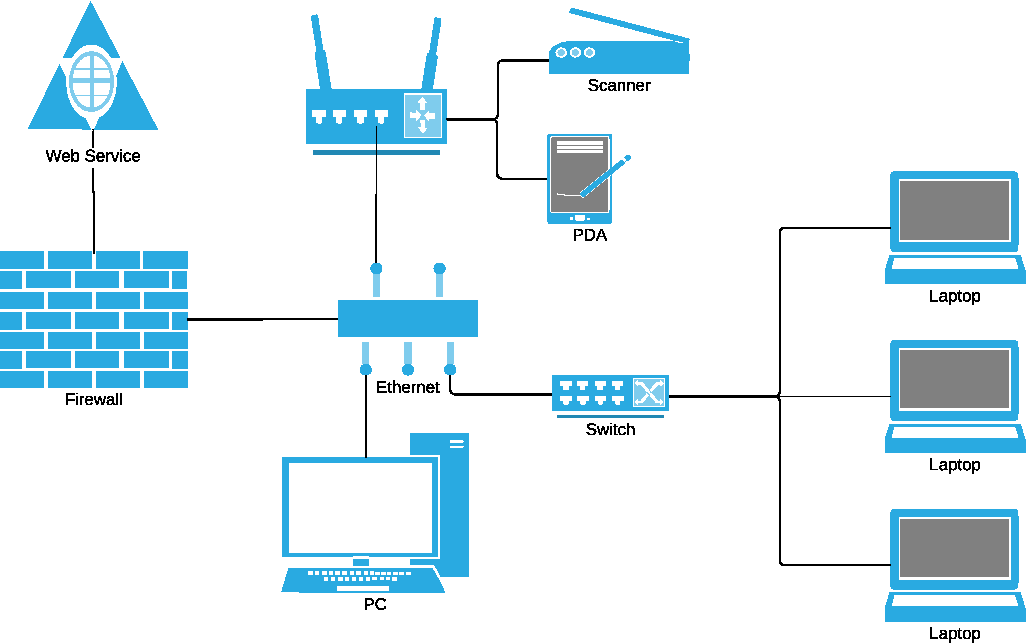
\includegraphics[width=.9\textwidth]{network} }%
    \mode<article>{ 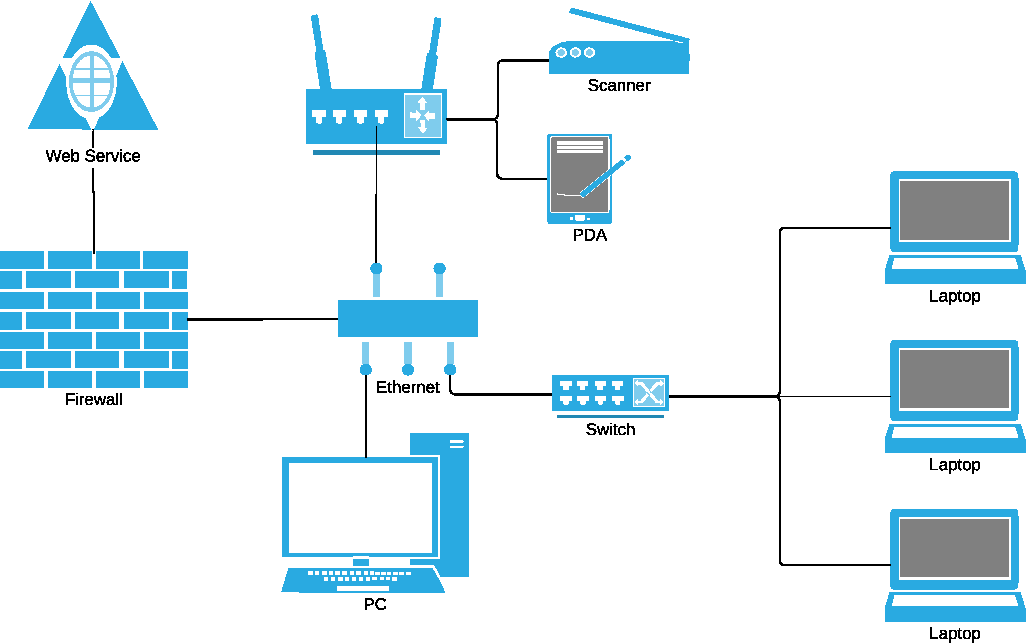
\includegraphics[width=.7\textwidth]{network} }
  \end{center}
\end{frame}

See also: \citetitle{wiki:network}

% \begin{frame}
%   \begin{center}
%     \mode<beamer>{ 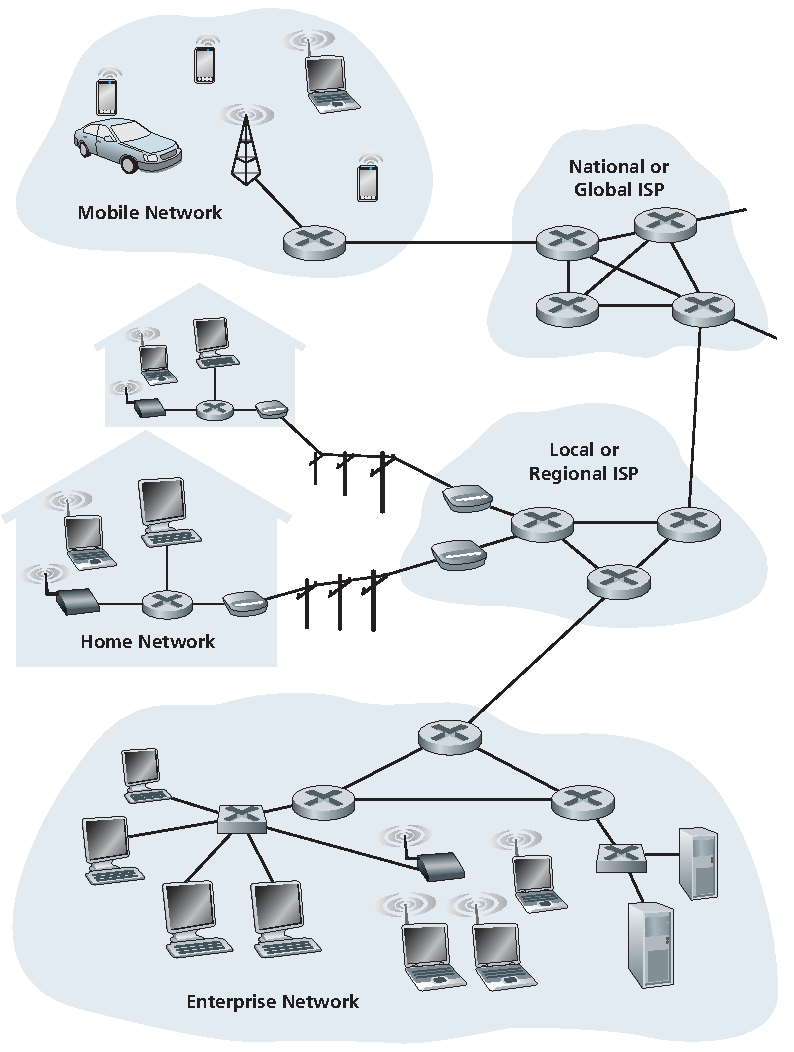
\includegraphics[height=\textheight]{internet} }%
%     \mode<article>{ 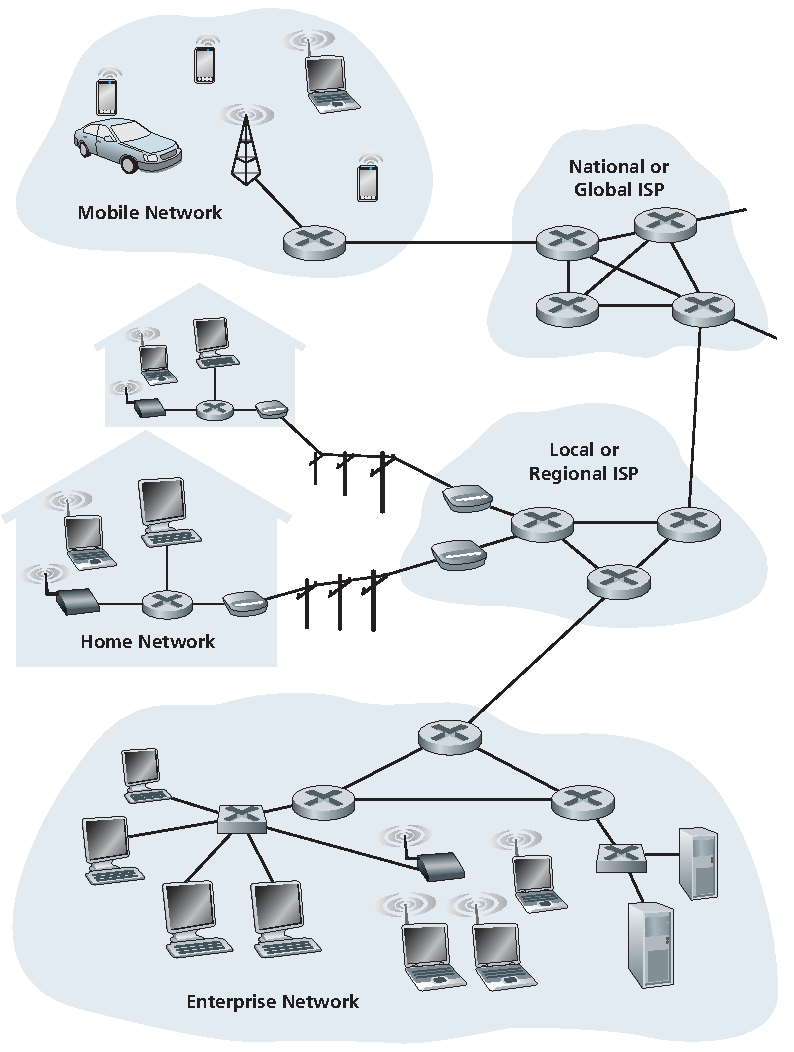
\includegraphics[width=.7\textwidth]{internet} }
%   \end{center}
% \end{frame}

\subsection[History]{Past and Future}

\begin{frame}[allowframebreaks=.8]{The History of Internet}
  \begin{description}
  \item[1836:] Telegraph
  \item[1858-66:] Transatlantic cable
  \item[1876:] Telephone
  \item[1957:] USSR launches Sputnik
  \item[1962-68:] \emph{Packet-switching} networks developed
  \item[1969:] Birth of Internet
  \item[1971:] People communicate over a network
  \item[1972:] Computers can connect more freely and easily
  \item[1973:] Global Networking becomes a reality
  \item[1974:] Packets become mode of transfer
  \item[1976:] Networking comes to many
  \item[1977:] E-mail takes off, Internet becomes a reality
  \item[1979:] News Groups born
  \item[1981:] Things start to come together
  \item[1982:] \emph{\tcpip{}} defines future communication
  \item[1983:] Internet gets bigger
  \item[1984:] Growth of Internet Continues
  \item[1986:] Power of Internet Realised
  \item[1987:] Commercialisation of Internet Born
  \item[1989:] Large growth in Internet
  \item[1990:] Expansion of Internet continues
  \item[1991:] Modernisation Begins
  \item[1992:] Multimedia changes the face of the Internet
  \item[1993:] The WWW Revolution truly begins
  \item[1994:] Commercialisation begins
  \item[1995:] Commercialisation continues apace
  \item[1996:] Microsoft enters
  \item[1998:] \includegraphics[height=.9em]{google}
  \item[Homework:] Meanwhile, what happened in China?
  \end{description}
\end{frame}

See also: \citetitle{rfc2235}

\subsection[Internet]{The Internet}

\begin{frame}{What's The Internet?}
  What pops up in your mind if I say ``Internet''?\pause
  
  \begin{iblock}{For me, the answer is...}
    \begin{center}
      \mode<beamer>{\includegraphics[width=.4\textwidth]{google} }%
      \mode<article>{\includegraphics[height=1em]{google} }
    \end{center}
      and...\pause
    \begin{center}
      \mode<beamer>{\Tcpip{}}%
      \mode<article>{\tcpip}
    \end{center}
  \end{iblock}
\end{frame}

See also: \citetitle{wiki:google, wiki:tcpip}

\begin{frame}{What's The Internet?}
  \begin{itemize}
  \item The network of networks.
  \item Tech view: \href{http://en.wikipedia.org/wiki/Tcp/ip}{{\tcpip}}
  \item App view: \href{http://en.wikipedia.org/wiki/Google}{\googlelogo}
  \end{itemize}
\end{frame}

\subsubsection[Why Google?]{Google Philosophy}

\begin{frame}{\googlelogo{} Philosophy}
  {\href{http://www.google.com/corporate/tenthings.html}{Ten things Google has found
      to be true}}

  \begin{enumerate}
  \item Focus on the user and all else will follow.
  \item It's best to do one thing really, really well.
  \item Fast is better than slow.
  \item Democracy on the web works.
  \item You don't need to be at your desk to need an answer.
  \item \emph{You can make money without doing evil.}
  \item There's always more information out there.
  \item The need for information crosses all borders.
  \item You can be serious without a suit.
  \item Great just isn't good enough.
  \end{enumerate}
\end{frame}

See also: \citetitle{wiki:evil}

\begin{frame}{\googlelogo{} Philosophy}{More about...}
  \begin{itemize}
  \item \href{http://www.google.com/corporate/software_principles.html}{Software Principles}
  \item \href{http://www.google.com/corporate/ux.html}{Google User Experience}
  \item \href{http://www.google.com/corporate/nopopupads.html}{No pop-ups}
  \item \href{http://www.google.com/corporate/security.html}{Security}
  \end{itemize}
\end{frame}

\subsubsection{Google Products}

\begin{frame}{\googlelogo{} Products}
  \begin{center}
    \mode<beamer>{ 
\includegraphics[width=.7\textwidth]{Google-Icons} }%
    \mode<article>{ 
\includegraphics[width=.1\textwidth]{Google-Icons} }
  \end{center}
\end{frame}

See also \citetitle{wiki:googleproducts}

\subsubsection[Browsers]{Choosing The Right Tools}

\begin{frame}{Choosing The Right Tools}
  \mode<beamer>{
    \begin{center}
      \begin{tabular}{c@{\qquad\qquad}c@{\qquad\qquad}c}
        \raisebox{1ex}{\scalebox{5}{\win}}%
        &
\includegraphics[height=5em]{linuxlogo}%
        &
\includegraphics[height=5em]{applelogo}\\
        &&\\
        &&\\
        \raisebox{2ex}{\scalebox{5}{\ie}}%
        &\includegraphics[height=5em]{firefox}%
        &
\includegraphics[height=5em]{gchrome}\\
        &&\\
        &&\\
        \scalebox{5}{\googleg}%
        &\textcolor{gray}{{\Huge vs.}}%
        &\scalebox{5}{\baidu}\hspace{-1.7em}\textbf{\LARGE\textcolor{white}{du}}
      \end{tabular}
    \end{center}}%
  \mode<article>{
    \begin{center}
      \begin{tabular}{ccc}
        \win[false] & \linux & \apple[false] \\\hline
        \ie[false] & \firefox & \chrome[false] \\\hline
        \googleg[false] & vs. & \baidu[false]
      \end{tabular}
    \end{center}}
\end{frame}

See also: \citetitle{wiki:ie, wiki:baidu}

\subsubsection{Safe Surfing}

\begin{frame}{Dangerous}
  \begin{center}
    \mode<beamer>{ 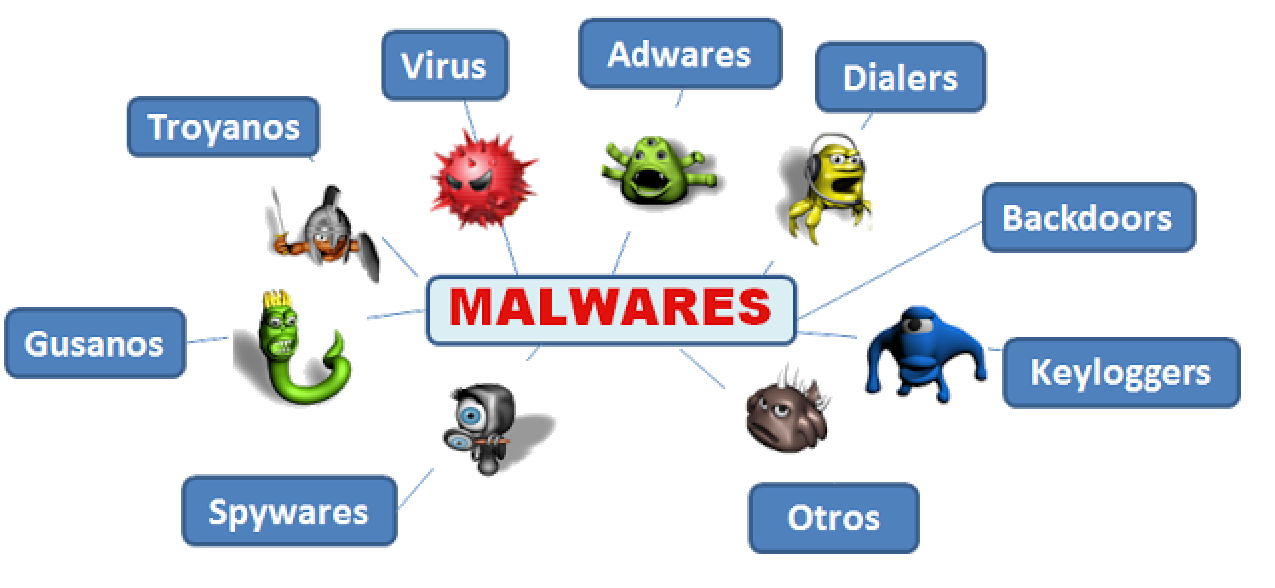
\includegraphics[width=\textwidth]{malware} }%
    \mode<article>{ 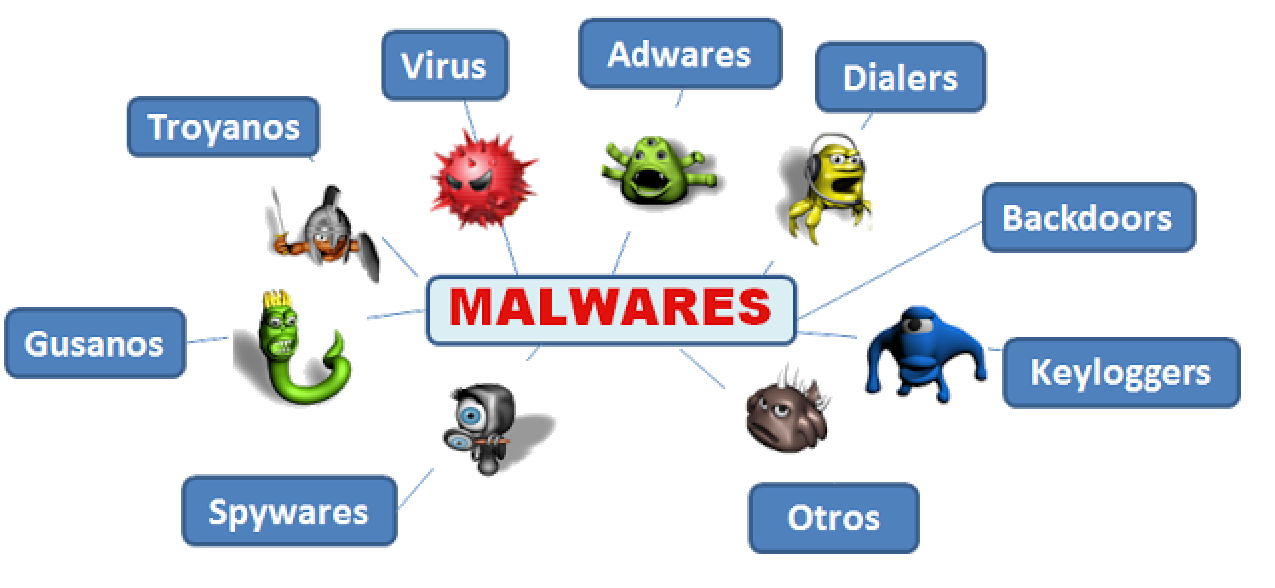
\includegraphics[width=.3\textwidth]{malware} }
  \end{center}\pause
  \begin{iblock}{My solution}
    \begin{center}
      
\includegraphics[height=5em]{linuxlogo}
    \end{center}
  \end{iblock}
\end{frame}

See also: \citetitle{wiki:malware, wiki:virus, wiki:adware, wiki:spyware, wiki:worm, wiki:trojan}
  

\begin{frame}{Safe Surfing Advice}{Take care of your identity and privacy}
  \begin{itemize}
  \item Use a better browser, and keep it updated
  \item Use a spam filter for emailing
  \item Always use strong passwords
  \item Don't give away too much personal information on blogs and social networking sites
  \end{itemize}
\end{frame}

\begin{frame}{Safe Surfing Advice}{Protect Your PC}
  \begin{itemize}
  \item Get anti-virus software, anti-spyware software and a firewall
  \item Keep your computer up to date
  \item Block spam emails
  \item Use an up to date web browser
  \item Make regular backups
  \item Encrypt your wireless network
  \end{itemize}
\end{frame}

\begin{frame}{Safe Surfing Advice}{Avoid online rip-offs}
  \begin{itemize}
  \item When you're shopping online, look for clear signs that you're buying from a reputable
    company
  \item On an online auction site, learn how it works and learn to pick good sellers
  \item Use safe ways to pay, such as PayPal or credit and debit cards
  \item Use your common sense to avoid scams – if it sounds too good to be true, it probably is
  \end{itemize}
\end{frame}

\begin{frame}{Homework}
  \begin{enumerate}
  \item try 
\includegraphics[height=1.5em]{linuxlogo}
  \item get a \href{https://mail.google.com}{gmail} account
  % \item recommend a good
  %   \href{https://chrome.google.com/webstore/category/apps?utm_source=chrome-ntp-icon}{chrome
  %   extension} to me via gmail
  % \item in \href{https://plus.google.com}{google plus}, share an interesting post to me
  \item add your class timetable into \href{https://calendar.google.com}{google calendar},
    and then share your calendar to me via gmail
  \item in \href{https://youtube.com}{youtube}, find a video you like and share it to me
  \end{enumerate}
\end{frame}


\lecture[Tutorial]{A Very Brief Internet Tutorial (II)}{tutorial}
%\mode<article>{\clearpage}
\section{How The Internet Works}

\subsection[Classification]{Network Classification}

\begin{frame}{Network Classification}
  \begin{itemize}
  \item connection method: wired, wireless...
  \item topology
  \item scale
  \item network architecture: c/s, p2p...
  \end{itemize}
\end{frame}

\begin{frame}{Network Classification}
  \begin{iblock}{Connection method}
    Wired:
    \begin{center}
      \mode<beamer>{
      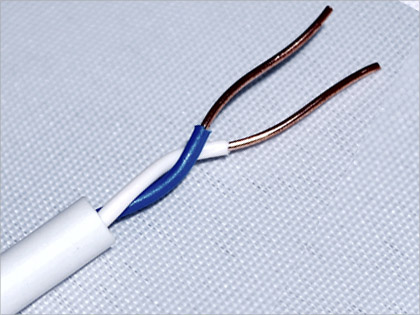
\includegraphics[height=1.6cm]{twisted-pair}\quad
      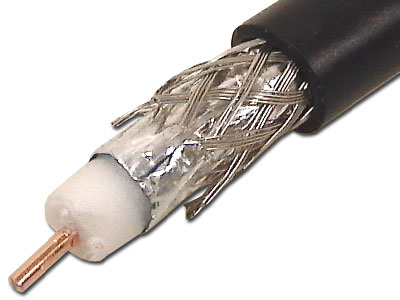
\includegraphics[height=1.6cm]{coaxial-cable}\quad
      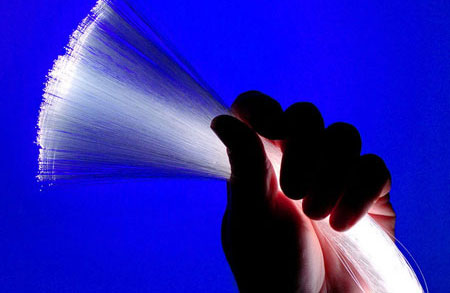
\includegraphics[height=1.6cm]{fiber-optics}}
    \mode<article>{
      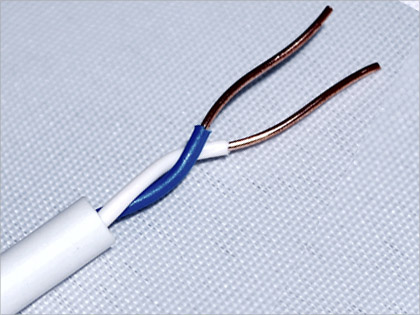
\includegraphics[height=1cm]{twisted-pair}\quad
      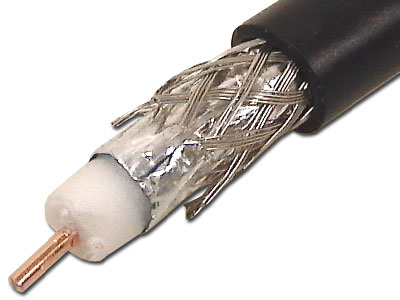
\includegraphics[height=1cm]{coaxial-cable}\quad
      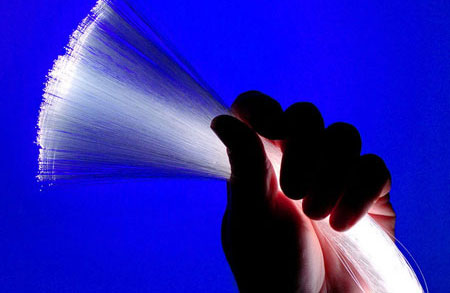
\includegraphics[height=1cm]{fiber-optics}}
    \end{center}
    Wireless:
    \begin{center}
      \mode<beamer>{
      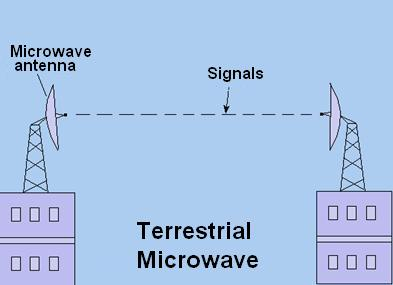
\includegraphics[height=1.6cm]{terrestrial}\quad
      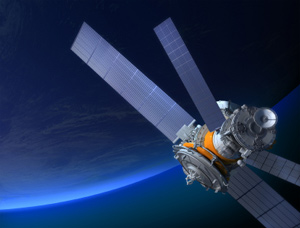
\includegraphics[height=1.6cm]{satellite}\quad
      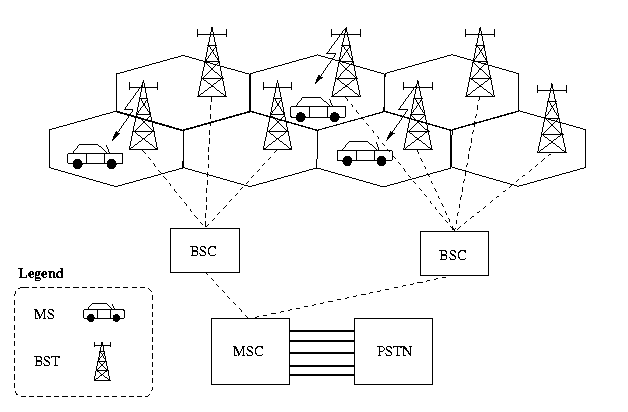
\includegraphics[height=1.6cm]{cellular}\\
      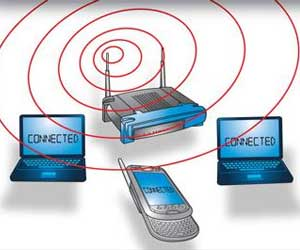
\includegraphics[height=1.6cm]{wlan}\quad
      
\includegraphics[height=1.6cm]{bluz}}
    \mode<article>{
      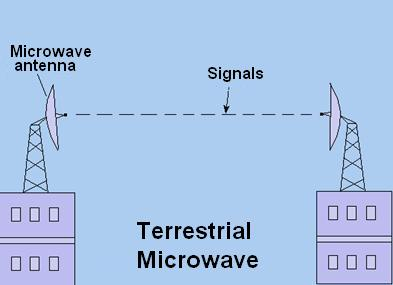
\includegraphics[height=1cm]{terrestrial}\quad
      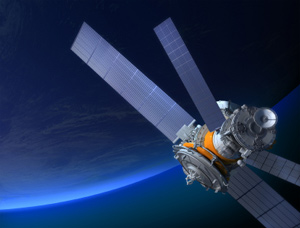
\includegraphics[height=1cm]{satellite}\quad
      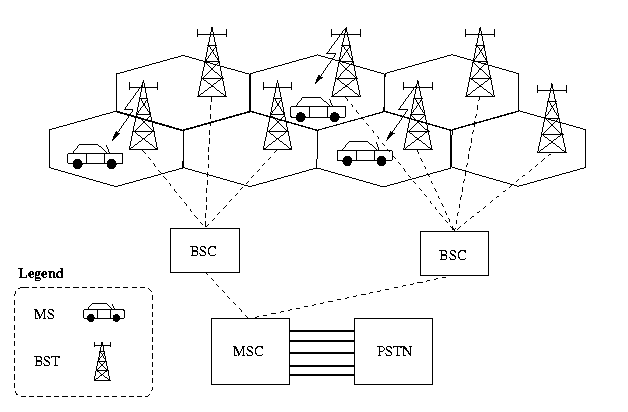
\includegraphics[height=1cm]{cellular}\\
      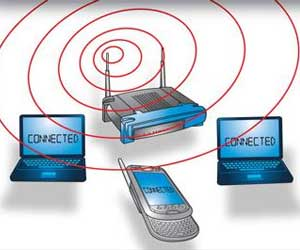
\includegraphics[height=1cm]{wlan}\quad
      
\includegraphics[height=1cm]{bluz}}
    \end{center}
  \end{iblock}
\end{frame}

\begin{frame}
  \begin{iblock}{Scale}
      \small{PAN}, \large{LAN}, \Large{CAN}, \LARGE{MAN}, \Huge{WAN} ...
  \end{iblock}
\end{frame}

\begin{frame}
  \begin{iblock}{Topology}
    \begin{center}
      \mode<beamer>{ 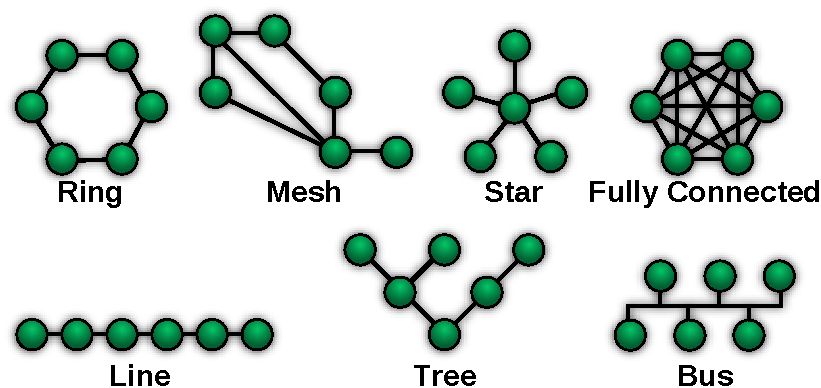
\includegraphics[width=\textwidth]{topo} }%
      \mode<article>{ 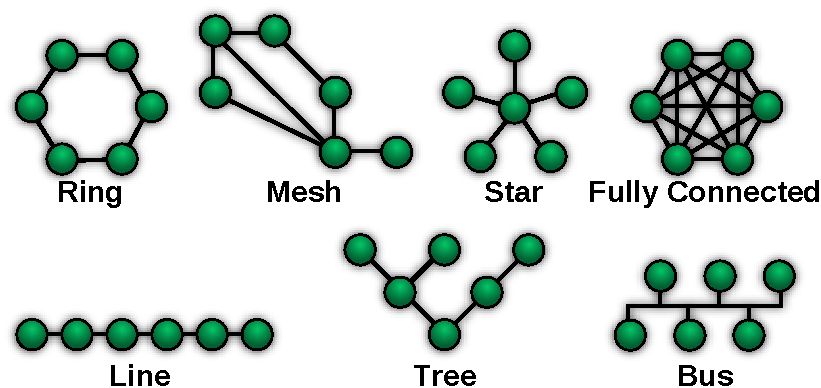
\includegraphics[width=.3\textwidth]{topo} }
    \end{center}
  \end{iblock}
\end{frame}

See also: \citetitle{wiki:topo}

\begin{frame}
  \begin{iblock}{Network Architecture}
    \begin{center}
      \mode<beamer>{ 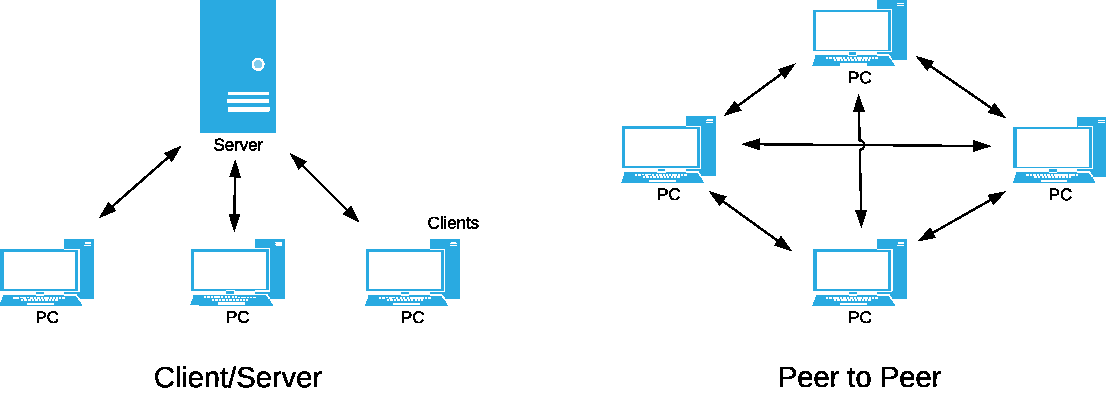
\includegraphics[width=\textwidth]{arch} }%
      \mode<article>{ 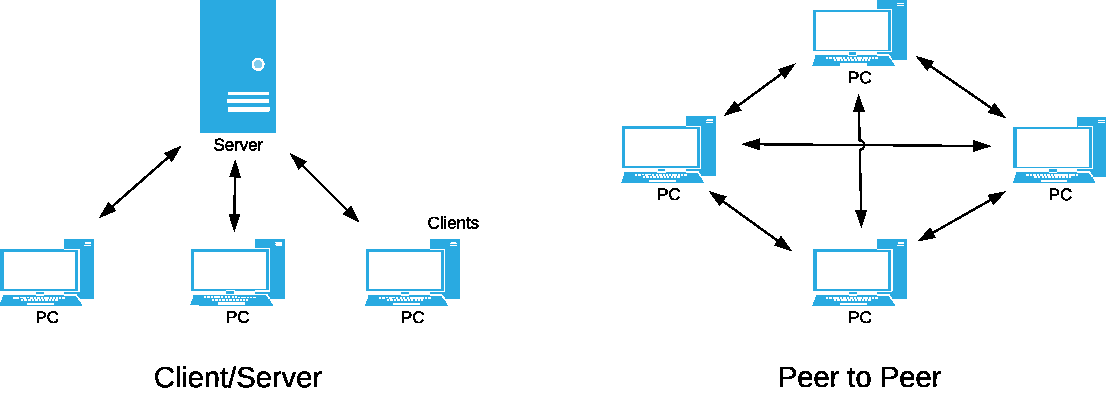
\includegraphics[width=.5\textwidth]{arch} }
    \end{center}
  \end{iblock}
\end{frame}

See also: \citetitle{wiki:netarch}

\subsection[Hardwares]{Basic Hardware Components}

\begin{frame}{Basic Hardware Components}
  \begin{center}
    \begin{tabular}{r|rlrlrl}\midrule
      IP&&&&&
      Router:&
\includegraphics[width=1cm]{router}\\\midrule
      Link&&&
      Bridge:&\raisebox{-7pt}{
\includegraphics[width=1cm]{bridge}}&
      Switch:&\raisebox{-7pt}{
\includegraphics[width=1cm]{cisco-switch}}\\\midrule
      PHY&NIC:&\raisebox{-5pt}{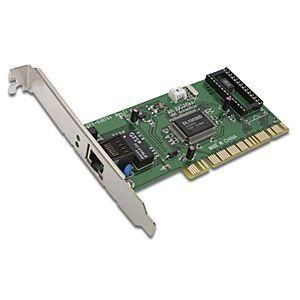
\includegraphics[width=1cm]{nic}}&
      Repeater:&\raisebox{-5pt}{
\includegraphics[width=1cm]{repeater}}&
      Hub:&\raisebox{-7pt}{
\includegraphics[width=1cm]{hub}}\\\midrule
    \end{tabular}
  \end{center}
\end{frame}

\subsection{Network Architecture}

\begin{frame}{\tcpip{}}
  \begin{center}
    \mode<beamer>{ \includegraphics[width=.6\textwidth]{basic-structure} }%
    \mode<article>{ \includegraphics[width=.2\textwidth]{basic-structure} }
  \end{center}
\end{frame}

See also: \citetitle{wiki:tcpip, rfc1180}

Each Internet-enabled computer has a TCP/IP protocol stack inside. And as you can see, the
incoming packets will face a 1-to-N situation. The value of the \emph{type} field in the
Ethernet frame determines whether the Ethernet frame is passed to the ARP or the IP
module. The \emph{protocol} field in the IP header, and the port number in TCP/UDP header
serve in a similar way.

\begin{frame}{What's {\tcpip{}}?}
  \begin{description}
  \item[TCP/IP] A set of protocols designed for the Internet
  \item[protocol] a rule, a treaty, an agreement ...
  \end{description}
  \begin{center}
    \mode<beamer>{ 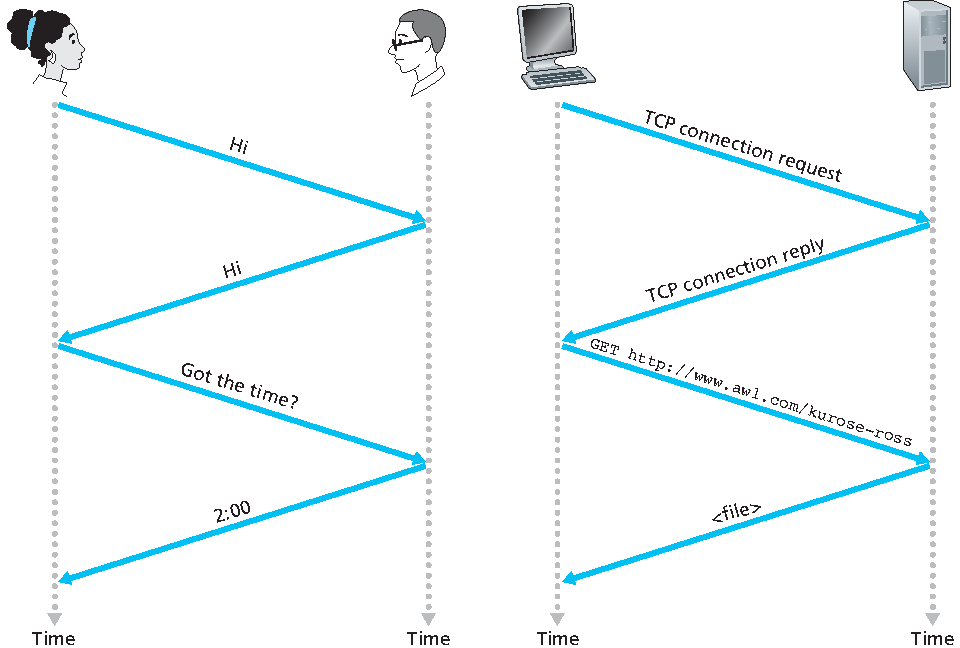
\includegraphics[width=.8\textwidth]{protocol} }%
    \mode<article>{ 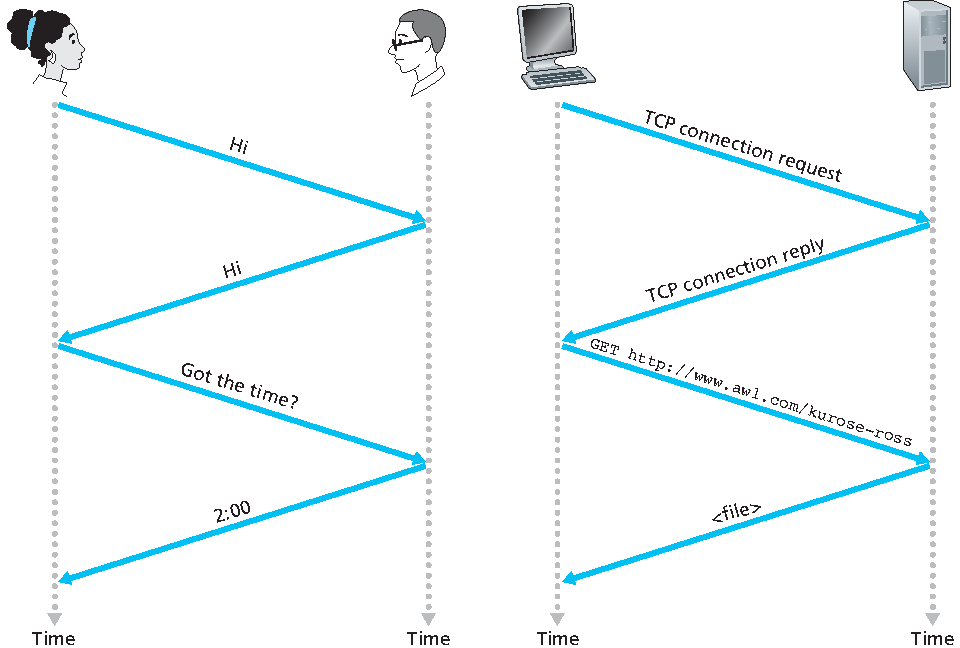
\includegraphics[width=.4\textwidth]{protocol} }
  \end{center}
\end{frame}

\begin{frame}{{\tcpip{}} Protocol Stack}
  \begin{iblock}{Every networked computer has it inside}
    \begin{center}
      \mode<beamer>{ 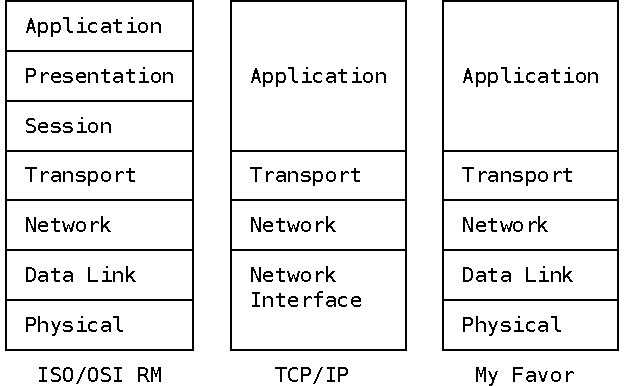
\includegraphics[width=.8\textwidth]{stack} }%
      \mode<article>{ \includegraphics[width=.4\textwidth]{stack} }
    \end{center}
  \end{iblock}
\end{frame}

See also: \citetitle[Sec.~1.3, \emph{Network Software}]{tanenbaum2011computer}.

TCP/IP means everything related to TCP and IP.

% \begin{frame}{Layered Design}
%   \begin{center}
%     \mode<beamer>{ \includegraphics[width=.8\textwidth]{layered-design} }%
%     \mode<article>{ \includegraphics[width=.4\textwidth]{layered-design} }
%   \end{center}
% \end{frame}

\begin{frame}{Layered Design}{Services vs. Protocols}
  \mode<beamer>{
    \begin{tikzpicture}[remember picture, overlay]
      \node [red,opacity=.3,anchor=north east,scale=.5,yshift=-2em] at (current page.north east)%
      {\includegraphics{layered-design}};
    \end{tikzpicture}}

  \mode<article>{
    \begin{minipage}{.35\linewidth}
      \includegraphics[width=\textwidth]{layered-design}
    \end{minipage}\quad
    \begin{minipage}{.6\linewidth}
      \includegraphics[width=\textwidth]{service-protocol}  
    \end{minipage}}
  
  \mode<beamer>{\includegraphics[width=.7\textwidth]{service-protocol}}%
  \begin{center}
    \begin{tabular}{c|c}\toprule
      \textbf{Services}&\textbf{Protocols}\\\midrule
      Layer to Layer&Peer to Peer\\\midrule
      A set of operations&A set of rules\\
      {\ttfamily\begin{tabular}{c}
                  (listen, connect, accept,\\
                  receive, send, disconnect) 
                \end{tabular}} &
                                 {\ttfamily\begin{tabular}{c}
                                             (message format,\\
                                             message meanings)
                                           \end{tabular}}\\\bottomrule
    \end{tabular}
  \end{center}
\end{frame}

See also: \citetitle[Sec.~1.3.5, \emph{The Relationship of Services to
  Protocols}]{tanenbaum2011computer}

\paragraph{Network architecture}

\begin{description}
\item[Architecture:] A big blueprint without worrying about any design details.
  \begin{itemize}
  \item A set of layers and protocols
  \item Neither the details of the implementation nor the specification of the interfaces
    is part of the architecture.
  \end{itemize}
\end{description}
  
\paragraph{Services}

Interfaces between layers (primitives, functions)
  % \begin{itemize}
  % \item[Q1.] Who provides which service to whom?
  % \item[Q2.] How this service is implemented?
  % \end{itemize}

\paragraph{Protocols}

\begin{itemize}
\item for peer to peer talking
\item The \emph{internal implementation} of services provided by a layer
\item It's common that different hosts use different implementations of the same protocols
  (e.g. Linux vs. Windows)
\item Protocol changes have no effects on it's upper/lower layers
\end{itemize}

\begin{frame}{Layered Design Example}
  \begin{iblock}{Taking an airplane trip}
    \begin{center}
      \mode<beamer>{ \includegraphics[width=.6\textwidth]{airtrip} }%
      \mode<article>{ \includegraphics[width=.3\textwidth]{airtrip} }
    \end{center}
    Each layer
    \begin{enumerate}
    \item has some functions
    \item provides services to its upper layer
    \end{enumerate}
  \end{iblock}
\end{frame}

See also:
\begin{itemize}
\item \citetitle[Sec.~1.5.1, \emph{Layered Architecture}]{kurose2013computer}
\item \citetitle[Sec.~1.3.2, \emph{Design Issues for the Layers}]{tanenbaum2011computer}
\end{itemize}

\paragraph{Layered design}

\begin{itemize}
\item Reduce design complexity
\item Serve as a black box to its upper layer
  \begin{itemize}
  \item Black box examples: information hiding, abstract data type, data encapsulation,
    object oriented programming
  \end{itemize}
\end{itemize}
  
\paragraph{Design issues}

\begin{itemize}
\item Reliability
  \begin{itemize}
  \item never lost data --- by means of acknowledgement
  \item Error detection/correction
  \item Routing
  \end{itemize}
\item Evolution
  \begin{itemize}
  \item Protocol layering
  \item Addressing
  \item Internetworking: disassembling, transmitting, reassembling
  \item Scalability
  \end{itemize}
\item Resource allocation
  \begin{itemize}
  \item Statistical multiplexing
  \item Flow control
  \item Congestion
  \item QoS
  \end{itemize}
\item Security
  \begin{itemize}
  \item Authentication
  \item Integrety
  \end{itemize}
\end{itemize}

See also \citetitle{rfc1122}.

\begin{frame}%{Layered Design}
  \begin{center}
    \mode<beamer>{ \includegraphics[height=\textheight]{trump-kim-en} }%translator
    \mode<article>{ \includegraphics[width=.6\textwidth]{trump-kim-en}}\label{fig:translator}%
  \end{center}
\end{frame}

\begin{frame}
  \begin{iblock}{Each protocol is completely independent of the other ones}
    For example
    \begin{itemize}
    \item The translators (L2) can switch from Chinese to Finnish without touching L1 or L3
    \item The secretaries (L1) can switch from fax to email without disturbing (or
      even informing) the other layers
    \end{itemize}
  \end{iblock}
\end{frame}

An analogy may help explain the idea of multilayer communication. Imagine two philosophers
(peer processes in layer 3), one of whom speaks Urdu and English and one of whom speaks
Chinese and French. Since they have no common language, they each engage a translator
(peer processes at layer 2), each of whom in turn contacts a secretary (peer processes in
layer 1). Philosopher 1 wishes to convey his affection for oryctolagus cuniculus to his
peer. To do so, he passes a message (in English) across the 2/3 interface to his
translator, saying ``I like rabbits,'' as illustrated in Fig.~\ref{fig:translator}. The
translators have agreed on a neutral language known to both of them, Dutch, so the message
is converted to ``Ik vind konijnen leuk.'' The choice of the language is the layer 2
protocol and is up to the layer 2 peer processes.\citetitle[Sec.~1.3, \emph{Network Software},
p.~31]{tanenbaum2011computer}

The translator then gives the message to a secretary for transmission, for example, by
email (the layer 1 protocol). When the message arrives at the other secretary, it is
passed to the local translator, who translates it into French and passes it across the 2/3
interface to the second philosopher. Note that each protocol is completely independent of
the other ones as long as the interfaces are not changed. The translators can switch from
Dutch to, say, Finnish, at will, provided that they both agree and neither changes his
interface with either layer 1 or layer 3. Similarly, the secretaries can switch from email
to telephone without disturbing (or even informing) the other layers. Each process may add
some information intended only for its peer. This information is not passed up to the
layer above.

\subsection{TCP/IP Overview}

\paragraph{Historical}

  The ARPANET was a research network sponsored by the DoD (U.S. Department of
  Defense). ...  When satellite and radio networks were added later, the existing
  protocols had trouble interworking with them, so a new reference architecture was
  needed. Thus, \emph{from nearly the beginning, the ability to connect multiple networks in
    a seamless way was one of the major design goals}.  This architecture later became
  known as the TCP/IP Reference Model, after its two primary protocols. \citetitle[Sec.~1.4.2,
  \emph{The TCP/IP Reference Model}]{tanenbaum2011computer}

  Given the DoD's worry that some of its precious hosts, routers, and internetwork
  gateways might get blown to pieces at a moment's notice by an attack from the Soviet
  Union, another major goal was that the network be able to survive loss of subnet
  hardware, without existing conversations being broken off. In other words, \emph{the DoD
    wanted connections to remain intact as long as the source and destination machines
    were functioning, even if some of the machines or transmission lines in between were
    suddenly put out of operation}. Furthermore, since applications with divergent
  requirements were envisioned, ranging from transferring files to real-time speech
  transmission, a flexible architecture was needed.


\begin{frame}{{\tcpip} Overview}{Basic Structure}
  \begin{minipage}{.4\linewidth}
    \includegraphics[width=\textwidth]{basic-structure}\label{fig:basic-node}
  \end{minipage}\hfill
  \begin{minipage}{.6\linewidth}
    \begin{enumerate}
    \item Where will an incoming Ethernet frame go?
      \begin{itemize}
      \item[] \texttt{0x0806} {\dejavu ➜} ARP
      \item[] \texttt{0x0800} {\dejavu ➜} IP
      \end{itemize}
    \item Where will an incoming IP packet go?
      \begin{itemize}
      \item[] \texttt{0x06} {\dejavu ➜} TCP
      \item[] \texttt{0x11} {\dejavu ➜} UDP
      \end{itemize}
    \item Where will an incoming transport message (UDP datagram, TCP segment) go?
      \begin{center}{\small
        \begin{tabular}{cccc}\hline
          HTTP&FTP&SSH&SMTP\\
          \texttt{80}&\texttt{21/20}&\texttt{22}&\texttt{25}\\\hline
        \end{tabular}}
      \end{center}
      % \begin{center}
      %   \begin{small}
      %     \tabulinesep=3pt
      %     \begin{tabu}spread 0pt{X[c]X[c]X[c]X[c]}\hline
      %       HTTP&FTP&SSH&SMTP\\
      %       \texttt{80}&\texttt{21/20}&\texttt{22}&\texttt{25}\\\hline
      %     \end{tabu}
      %   \end{small}
      % \end{center}
    \end{enumerate}
  \end{minipage}
\end{frame}

\subsection{Terminology}
  
\begin{frame}{The Name Of A Unit Of Data}
  \vspace*{-5em}
  \begin{minipage}{.4\linewidth}
    \begin{itemize}
    \item[A] Application message
    \item[T] TCP segment; UDP datagram
    \item[N] IP packet
    \item[L] Ethernet frame
    \end{itemize}
  \end{minipage}\hfill
  \begin{minipage}{.6\linewidth}
    \begin{center}
      \mode<beamer>{ \includegraphics[width=\columnwidth]{encap} }%
      \mode<article>{ \includegraphics[width=.7\columnwidth]{encap} }
    \end{center}
  \end{minipage}
  \mode<beamer>{
    \begin{tikzpicture}[remember picture, overlay]
      \node (a) [red,opacity=.3,anchor=south west,scale=.4] at (current page.south west)%
      {\includegraphics{basic-structure}};
      \node (b) [red,opacity=.3,right=.5cm of a,scale=.4,yshift=-3cm] {\includegraphics{indirect-routing-2}};
    \end{tikzpicture}}
\end{frame}

\subsection{Ethernet}
  
\begin{frame}\mode<beamer>{\frametitle{Ethernet}}
  \begin{center}
    \mode<beamer>{\includegraphics[width=\textwidth]{eth}}%
    \mode<article>{\includegraphics[width=.6\textwidth]{eth}}
  \end{center}
  \begin{enumerate}
  \item Frame format?
  \item Address format?
  \item Broadcast address?
  \item CSMA/CD?
  \end{enumerate}
\end{frame}

\begin{frame}{Ethernet Frame}
  \begin{center}
    \mode<beamer>{ \includegraphics[width=.65\textwidth]{ethhdr} }%
    \mode<article>{ \includegraphics[width=.3\textwidth]{ethhdr} }
  \end{center}
\end{frame}

\begin{frame}{Examples}
  \begin{iblock}{Unicast, carrying an IP packet}
    \mode<beamer>{\includegraphics[width=\textwidth]{ethframe3}}%
    \mode<article>{\includegraphics[width=.6\textwidth]{ethframe3}}
  \end{iblock}
  \begin{iblock}{Unicast, carrying an ARP packet}
    \mode<beamer>{\includegraphics[width=\textwidth]{ethframe2}}%
    \mode<article>{\includegraphics[width=.6\textwidth]{ethframe2}}
  \end{iblock}
  \begin{iblock}{Broadcast, carrying an ARP packet}
    \mode<beamer>{\includegraphics[width=\textwidth]{ethframe}}%
    \mode<article>{\includegraphics[width=.6\textwidth]{ethframe}}
  \end{iblock}
\end{frame}

\begin{description}
\item[CSMA/CD] CSMA/CD is the communication protocol used by devices in the same Ethernet
  when they talk to each other.
  \begin{itemize}
  \item \emph{Carrier Sense} means every device in the Ethernet can detect whether the
    carrier is busy. Carrier, the media used for carrying electric signals, is the Ethernet cable;
  \item \emph{Multiple Access} means every device has equal chance of using the carrier
    for data transmission ;
  \item \emph{Collision Detection} means if more than one devices trying to transmit
    data at the same time, they can detect this collision, and wait for a random (but
    short) period before trying to transmit again.
  \end{itemize}
  See \citetitle[Sec. 3.1]{rfc1180} for a human analogy.
\end{description}

\begin{frame}{Ethernet References}
  \begin{refsection}
  \nocite{wiki:ethernet,wiki:ethframe,wiki:csmacd,rfc1042} \printbibliography[heading=none]
\end{refsection}
\end{frame}

\subsection{ARP}

\begin{frame}\mode<beamer>{\frametitle{ARP}}
  \begin{description}
  \item[ARP] Looking up the ARP table to find the destination MAC address.
  \end{description}
  \begin{iblock}{Example ARP table}
    \hspace{2em}{\ttfamily
      \begin{tabular}{lr}
        \toprule
        \textrm{IP address} & \textrm{Ethernet address}\\\midrule
        223.1.2.1 & 08-00-39-00-2F-C3\\
        223.1.2.3 & 08-00-5A-21-A7-22\\
        223.1.2.4 & 08-00-10-99-AC-54\\\bottomrule
      \end{tabular}}
  \end{iblock}
  \mode<beamer>{
    \begin{tikzpicture}[remember picture, overlay]
      \node [red,opacity=.3,anchor=south east,scale=.7] at (current page.south east)%
      {\includegraphics{basic-structure}};
    \end{tikzpicture}}
\end{frame}

\begin{frame}{Where does the ARP table come from?}
  \begin{iblock}{Example ARP Request}
    \begin{center}
      \begin{tabular}{l>{\ttfamily}r}
        \toprule
        Sender IP Address & 223.1.2.1\\
        Sender Eth Address & 08-00-39-00-2F-C3\\\midrule
        Target IP Address & 223.1.2.2\\
        Target Eth Address & FF-FF-FF-FF-FF-FF\\\bottomrule
      \end{tabular}
    \end{center}
  \end{iblock}

  \begin{iblock}{Example ARP Response}
    \begin{center}
      \begin{tabular}{l>{\ttfamily}r}
        \toprule
        Sender IP Address &  223.1.2.2\\
        Sender Eth Address & 08-00-28-00-38-A9\\\midrule
        Target IP Address &  223.1.2.1\\
        Target Eth Address & 08-00-39-00-2F-C3\\\bottomrule
      \end{tabular}
    \end{center}
  \end{iblock}
  \mode<beamer>{
  \begin{tikzpicture}[remember picture, overlay]
    \node [red,opacity=.3,anchor=south east,scale=.4] at (current page.south east)%
    {\includegraphics{basic-structure}};
  \end{tikzpicture}}
\end{frame}
  
\begin{frame}%{ARP}{Where does the ARP table come from?}
  \begin{iblock}{The updated table}
    \begin{center}{\ttfamily
      \begin{tabular}{lr}
        \toprule
        \textrm{IP address} & \textrm{Ethernet address}\\\midrule
        223.1.2.1 & 08-00-39-00-2F-C3\\
        223.1.2.2 & 08-00-28-00-38-A9\\
        223.1.2.3 & 08-00-5A-21-A7-22\\
        223.1.2.4 & 08-00-10-99-AC-54\\\bottomrule
      \end{tabular}}
    \end{center}
  \end{iblock}
  \mode<beamer>{
  \begin{tikzpicture}[remember picture, overlay]
    \node [red,opacity=.3,anchor=south east,scale=.5] at (current page.south east)%
    {\includegraphics{basic-structure}};
  \end{tikzpicture}}
\end{frame}

\begin{frame}{ARP References}
  \begin{refsection}
  \nocite{wiki:arp, rfc826} \printbibliography[heading=none]
\end{refsection}
\end{frame}

\subsection{IP}

\begin{frame}\mode<beamer>{\frametitle{IP}\framesubtitle{Router}}
  \begin{minipage}{.45\linewidth}
    \begin{center}
      \mode<beamer>{ \includegraphics[width=\columnwidth]{basic-structure} }%
      \mode<article>{ \includegraphics[width=.7\columnwidth]{basic-structure} }
    \end{center}
  \end{minipage}\hfill
  \begin{minipage}{.45\linewidth}
    \begin{center}
      \mode<beamer>{ \includegraphics[width=\columnwidth]{basic-structure-2} }%
      \mode<article>{ \includegraphics[width=.7\columnwidth]{basic-structure-2} }
      \label{fig:router}
    \end{center}
  \end{minipage}
  \begin{description}
  \item[Routing] Find a route in the route table.
  \end{description}
\end{frame}

\begin{frame}{Direct Routing---IP is overhead}
    \begin{center}
      \mode<beamer>{ \includegraphics[height=.3\textheight]{direct-routing} }%
      \mode<article>{ \includegraphics[width=.2\textwidth]{direct-routing} }
    \end{center}
  \begin{iblock}{Addresses in an Ethernet frame for an IP packet from A to B}
    \begin{center}
      \begin{tabular}{ccc}
        \toprule
        address & source & destination\\\midrule
        IP & A & B\\
        Eth & A & B\\\bottomrule
      \end{tabular}
    \end{center}
  \end{iblock}
\end{frame}

\begin{frame}{Is IP Necessary?}
  \begin{center}
    \includegraphics[width=.25\textwidth]{without-ip}\qquad
    \includegraphics[width=.25\textwidth]{with-ip}\\[1em]
    \includegraphics[width=.25\textwidth]{dual-stack}
  \end{center}
\end{frame}

\begin{frame}{Indirect Routing}
  \begin{center}
    \mode<beamer>{ \includegraphics[width=.9\textwidth]{indirect-routing} }%
    \mode<article>{ \includegraphics[width=.5\textwidth]{indirect-routing} }
  \end{center}
  \label{fig:indirect-routing}
  \mode<beamer>{
    \begin{tikzpicture}[remember picture, overlay]
      \node [scale=.5,text opacity=.8,xshift=-60mm, yshift=-40mm] at (current page.center)
      {\includegraphics{basic-structure-2}};
    \end{tikzpicture}}
\end{frame}

\begin{frame}
  \begin{iblock}{Addresses in an Ethernet frame for an IP packet from A to E (before D)}
    \begin{center}
      \begin{tabular}{ccc}
        \toprule
        address & source & destination\\\midrule
        IP & A & E \\
        Eth & A & D \\\bottomrule
      \end{tabular}
    \end{center}
  \end{iblock}
  \begin{iblock}{Addresses in an Ethernet frame for an IP packet from A to E (after D)}
    \begin{center}
      \begin{tabular}{ccc}
        \toprule
        address & source & destination\\\midrule
        IP & A & E \\
        Eth & D & E \\\bottomrule
      \end{tabular}
    \end{center}
  \end{iblock}
  \mode<beamer>{
    \begin{tikzpicture}[remember picture, overlay]%
      \node [opacity=.2,anchor=center,scale=.8,yshift=-1ex] at (current page.south)
      {\includegraphics{indirect-routing}};
    \end{tikzpicture}}
\end{frame}

\begin{frame}{IP Module Routing Rules}
  \begin{minipage}{.8\linewidth}
  \begin{enumerate}
  \item For an outgoing IP packet, entering IP from an upper layer, IP must decide
    \begin{itemize}
    \item whether to send the IP packet directly or indirectly, and
    \item IP must choose a lower network interface.
    \end{itemize}
    These choices are made by consulting the route table.
  \item For an incoming IP packet, entering IP from a lower interface, IP must decide
    \begin{itemize}
    \item whether to forward the IP packet or pass it to an upper layer.
    \item If the IP packet is being forwarded, it is treated as an outgoing IP packet.
    \end{itemize}
  \item When an incoming IP packet arrives it is never forwarded back out through the same
    network interface.
  \end{enumerate}
\end{minipage}
\mode<beamer>{
  \begin{tikzpicture}[remember picture, overlay] \node [red,opacity=.3,scale=.45,anchor=east]
    at (current page.east) {\includegraphics{basic-structure-2}};
  \end{tikzpicture}}
\end{frame}

\begin{frame}{IP Address}
\begin{center}
  \mode<beamer>{ \includegraphics[width=\textwidth]{ipv4addr172} }%
  \mode<article>{ \includegraphics[width=.6\textwidth]{ipv4addr172} }
\end{center}
\end{frame}

\begin{frame}%{IP Address}
  \begin{iblock}{Address classes}
    \begin{center}
      \mode<beamer>{ \includegraphics[width=\textwidth]{ipv4addr} }%
      \mode<article>{ \includegraphics[width=.6\textwidth]{ipv4addr} }
    \end{center}
  \end{iblock}
\end{frame}

\begin{frame}{Prefix}
\begin{center}
  \mode<beamer>{\includegraphics[width=\textwidth]{prefix2}}%
  \mode<article>{\includegraphics[width=.7\textwidth]{prefix2}}
\end{center}
\end{frame}

\begin{frame}{Special IP Addresses}
  \begin{itemize}
  \item A value of zero in the network field means this network. (source only)
  \item A value of zero in the host field means network address.
  \item \texttt{127.x.x.x} are loopback address.
  \item \texttt{255.255.255.255} is boardcast address.
  \item Private address:
    \begin{itemize}
    \item \texttt{10.x.x.x}
    \item \texttt{172.16.x.x}$\sim$\texttt{172.31.x.x}
    \item \texttt{192.168.x.x}
    \end{itemize}
  \item CIDR---Classless Inter-Domain Routing---An IP addressing scheme that replaces the older
    system based on classes A, B and C.
  \end{itemize}
\end{frame}

See also: \citetitle[\emph{RFC 943}]{rfc943}

\begin{frame}{Names}
  People refer to computers by names, not numbers.
  \begin{iblock}{\texttt{/etc/hosts}}
    \begin{center}{\ttfamily
      \begin{tabular}{lll}
        127.0.0.1 & localhost&\\
        202.203.132.245 & cs3.swfu.edu.cn & cs3\\
      \end{tabular}}
    \end{center}
  \end{iblock}

  \begin{iblock}{\texttt{/etc/networks}}
    \begin{center}
      \texttt{localnet}\qquad \texttt{202.203.132.192}
    \end{center}
  \end{iblock}
\end{frame}

\begin{frame}{IP Route Table}
  \begin{iblock}{Example IP Route Table}
    \begin{center}
      \mode<beamer>{ \includegraphics[width=.7\textwidth]{route-table} }%
      \mode<article>{ \includegraphics[width=.3\textwidth]{route-table} }
    \end{center}
  \end{iblock}
  \begin{itemize}
  \item[\char`~\$] \texttt{man route}
  \end{itemize}
\end{frame}

\begin{frame}{Direct Routing Details}
  \begin{center}
    \mode<beamer>{ \includegraphics[height=.5\textheight]{direct-routing-2} }%
    \mode<article>{ \includegraphics[width=.3\textwidth]{direct-routing-2} }
  \end{center}

  \begin{iblock}{The route table inside alpha (simplified)}
    \begin{center}
      \begin{tabular}{llcc}
        \toprule
        network & flag & router & interface\\\midrule
        \texttt{development} & \texttt{direct} & & \texttt{1}\\\bottomrule
      \end{tabular}
    \end{center}
  \end{iblock}
\end{frame}

\begin{frame}{Homework}
  \begin{center}
    \includegraphics[width=\textwidth]{eth}\\[2em]
    Alpha is sending an IP packet to beta\ldots{}Please describe.
  \end{center}
\end{frame}
  
\begin{frame}{Indirect Routing Details}\label{indirect-routing-2}
  \begin{center}
    \mode<beamer>{ \includegraphics[width=\textwidth]{indirect-routing-2} }%
    \mode<article>{ \includegraphics[width=.75\textwidth]{indirect-routing-2} }
  \end{center}
\end{frame}

\begin{frame}{Indirect Routing Details}
  \begin{iblock}{The route table inside alpha}
    \begin{center}{\ttfamily
      \begin{tabular}{llcc}
        \toprule
        \textrm{network} & \textrm{flag} & \textrm{router} & \textrm{interface}\\\midrule
        223.1.2 & direct & & 1\\
        223.1.3 & indirect & 223.1.2.4 & 1\\
        223.1.4 & indirect & 223.1.2.4 & 1\\\bottomrule
      \end{tabular}}
    \end{center}
  \end{iblock}

  \begin{iblock}{The route table inside delta}
    \begin{center}{\ttfamily
      \begin{tabular}{llcc}
        \toprule
        \textrm{network} & \textrm{flag} & \textrm{router} & \textrm{interface} \\\midrule
        223.1.2 & direct & & 1\\
        223.1.3 & direct & & 3\\
        223.1.4 & direct & & 2\\\bottomrule
      \end{tabular}}
    \end{center}
  \end{iblock}
  \mode<beamer>{%
  \begin{tikzpicture}[remember picture, overlay]
    \node [scale=.5,opacity=.1,red,anchor=south] at (current page.south)
    {\includegraphics{indirect-routing-2}};%
  \end{tikzpicture}}
\end{frame}

\begin{frame}<beamer>{Homework}
  Alpha is sending an IP packet to epsilon\ldots{}Please describe.
  \begin{tikzpicture}[remember picture, overlay]
    \node [scale=.5,opacity=.2,red] at (current page.center)
    {\includegraphics{indirect-routing-2}};%
  \end{tikzpicture}
\end{frame}

\begin{frame}{Managing The Routes}
  \begin{itemize}
  \item Manually maintained by administrator
  \item ICMP can report some routing problems
  \item For larger networks, routing protocols are used.
  \end{itemize}
\end{frame}

\begin{frame}{IP Packet}
  \begin{center}
    \mode<beamer>{ \includegraphics[width=\textwidth]{ipv4-hdr} }%
    \mode<article>{ \includegraphics[width=.5\textwidth]{ipv4-hdr} }
  \end{center}
\end{frame}

\begin{frame}{IP References}
  \begin{refsection}
    \nocite{wiki:ip, wiki:ipaddr, rfc791, wiki:ipv4hdrchksum} \printbibliography[heading=none]
  \end{refsection}
\end{frame}

% \begin{frame}{SWFU Campus Network Topology}
%   \begin{center}
%     \mode<beamer>{
%       \includegraphics[width=\textwidth]{swfc_net_topo}
%     } \mode<article>{
%       \includegraphics[width=.8\textwidth]{swfc_net_topo}
%     }
%   \end{center}
% \end{frame}

% \begin{frame}{SWFU Campus Network Topology}
%   \begin{center}
%     \mode<beamer>{
%       \includegraphics[height=.9\textheight]{swfu-topo}
%     } \mode<article>{
%       \includegraphics[width=.8\textwidth]{swfu-topo}
%     }
%   \end{center}
% \end{frame}

% \begin{frame}
%   \begin{center}
%     \mode<beamer>{
%       \includegraphics[width=\textwidth]{D-topology}
%     } \mode<article>{
%       \includegraphics[width=.8\textwidth]{D-topology}
%     }
%   \end{center}
% \end{frame}

\subsection{Subnetting}

\begin{frame}{Why Subnetting?}
  \mode<beamer>{
    \begin{tikzpicture}[remember picture, overlay]
      \node [scale=.7,anchor=north east] at (current page.north east)
      {\includegraphics{addrcls-pie}};%
    \end{tikzpicture}}
  \begin{itemize}
  \item save address space
  \item restrict collision domain
  \item security
  \item physical media (Ethernet, FDDI, \ldots)    
  \end{itemize}
  \mode<beamer>{\includegraphics[width=.7\textwidth]{cls-hosts2} }%
  \mode<article>{ \includegraphics[width=.5\textwidth]{cls-hosts2} }
\end{frame}

\begin{frame}{How}
  \begin{center}
    \mode<beamer>{ \includegraphics[width=\textwidth]{subnetting} }%
    \mode<article>{ \includegraphics[width=.5\textwidth]{subnetting} }
  \end{center}
  \begin{description}
  \item[Subnet mask] is a bitmask used to identify the network and node parts of the address.
  \end{description}
  \begin{iblock}{Default Subnet Masks}
    \begin{tabular}{l>{\ttfamily}l>{\ttfamily}l}
      Class A & 255.0.0.0 &     11111111.0.0.0\\
      Class B & 255.255.0.0 &   11111111.11111111.0.0\\
      Class C & 255.255.255.0 & 11111111.11111111.11111111.0
    \end{tabular}
  \end{iblock}
\end{frame}

\begin{frame}{Example}
  \mode<beamer>{
    \begin{tikzpicture}[remember picture, overlay]
      \node [scale=.55,opacity=.7,red,anchor=east] at (current page.east)
      {\includegraphics{hierarchy-subnet}};%
      \node [font=\ttfamily,anchor=south west] at (current page.south west) {
        \begin{tabular}{rl@{.}l@{.}l@{.}l}
          CS:&10000000&11010000&1xxxxxxx&xxxxxxxx\\
          EE:&10000000&11010000&00xxxxxx&xxxxxxxx\\
          ART:&10000000&11010000&011xxxxx&xxxxxxxx\\
        \end{tabular}};
    \end{tikzpicture}}
  \vspace*{-.5em}
  \mode<beamer>{ \hspace{-1cm}\includegraphics[width=.9\textwidth]{subnetting-example} }%
  \begin{center}
    \mode<article>{ \includegraphics[width=.6\textwidth]{subnetting-example} }
  \end{center}
  \mode<article>{\ttfamily
    \begin{tabular}{rl@{.}l@{.}l@{.}l}
      CS:&10000000&11010000&1xxxxxxx&xxxxxxxx\\
      EE:&10000000&11010000&00xxxxxx&xxxxxxxx\\
      ART:&10000000&11010000&011xxxxx&xxxxxxxx\\
    \end{tabular}}
\end{frame}

See detailed explanation in \citetitle[P.445]{tanenbaum2011computer}.

\begin{frame}{$\mathbf{2^n-2}$}
  \begin{iblock}{Example}
    \begin{tabular}{r>{\ttfamily}c}\toprule
      IP address:&\begin{tabular}{c@{.}c@{.}c@{.}c}
                    11001010&11001011&10000100&11110001\\
                    202&203&132&241
                  \end{tabular}\\\midrule
      Subnet mask:&\begin{tabular}{c@{.}c@{.}c@{.}c}
                     11111111&11111111&11111111&11000000\\
                     255&255&255&192
                   \end{tabular}\\\bottomrule
    \end{tabular}
  \end{iblock}

  \begin{itemize}
  \item There are $2^2-2 = 2$ subnets
  \item Each subnet has $2^6-2 = 62$ nodes
  \item Subtract 2? All ``0''s and all ``1''s. (old story)
  \end{itemize}
\end{frame}

\begin{frame}{Subnet Calculator}
  \begin{iblock}{free IP subnet calculators}
    Try:
    \begin{itemize}
    \item[\char`~\$]  \texttt{subnetcalc 202.203.132.244/26}
    \item[\char`~\$]  \texttt{ipcalc 202.203.132.244/26}
    \item[\char`~\$]  \texttt{sipcalc 202.203.132.244/26}
    \end{itemize}
  \end{iblock}
\end{frame}

\begin{frame}{Quiz}
  \begin{center}
    \mode<beamer>{ \includegraphics[width=.8\textwidth]{subnetting-example} }%
    \mode<article>{ \includegraphics[width=.6\textwidth]{subnetting-example} }
  \end{center}
  Consider a packet addressing \texttt{128.208.2.251}
  \begin{itemize}
  \item[Q1:] Which subnet it belongs to?
  \item[Q2:] The route table inside each router?
  \end{itemize}
\end{frame}

\begin{frame}{Subnetting References}
  \begin{refsection}
    \nocite{wiki:subnet, wiki:ipv4subnetref,wiki:privatenet,rfc917,rfc950}
    \printbibliography[heading=none]
  \end{refsection}
\end{frame}

\subsection{CIDR}

\begin{frame}{CIDR---Classless Inter-Domain Routing}
  \begin{description}
  \item[CIDR] An IP addressing scheme that replaces the older system
    based on classes A, B and C.
  \end{description}
  \begin{iblock}{Why?}
    With a new network being connected to the Internet every 30 minutes the Internet was
    faced with two critical problems:
    \begin{itemize}
    \item Running out of IP addresses
    \item Running out of capacity in the global routing tables
    \end{itemize}
  \end{iblock}
\end{frame}

From \url{https://searchnetworking.techtarget.com/definition/CIDR}:
\begin{quote}
  CIDR is a more flexible way to allocate IP addresses than the original scheme. As a
  result, the number of IP addresses was greatly increased, which along with widespread
  use of network address translation (NAT), has significantly extended the useful life of
  IPv4.
\end{quote}

\begin{frame}{Two-Level Internet}{Network -- Host}
\begin{center}
  \includegraphics[width=\textwidth]{2-level-internet}
\end{center}
\end{frame}

\begin{frame}{Running out of IP addresses}
  Using the old addressing scheme, the Internet could support:
  \begin{itemize}
  \item 126 Class A networks that could include up to 16,777,214 hosts each
  \item Plus 65,000 Class B networks that could include up to 65,534 hosts each
  \item Plus over 2 million Class C networks that could include up to 254 hosts each
  \end{itemize}
  only 3\% of the assigned addresses were actually being used.
\end{frame}

The old classful scheme was very inefficient in IP address allocation especially in class
B. As we can imagine, for an medium-sized business, class A is too large, while class C is
too small. So usually class B is the choice though it still is far too large for most
organizations. In reality, more than half of class B networks have fewer than 50
hosts. Obviously, a class C network would have done the job, but everyone that asked for a
class B network thought his business would outgrow the 8-bit host field.

To handle this problem, subnets were introduced to flexibly assign blocks of addresses within an
organization.

\begin{frame}{Global Routing Tables At Capacity}
  \begin{itemize}
  \item As the number of networks on the Internet increased, so did the number of routes.
  \item A few years back it was forecasted that the global backbone Internet routers were
    fast approaching their limit on the number of routes they could support.
  \item Even using the latest router technology, the maximum theoretical routing table
    size is approximately 60,000 routing table entries.
  \item If nothing was done the global routing tables would have reached capacity by
    mid-1994 and all Internet growth would be halted.
  \end{itemize}
\end{frame}

Subnetting can significantly improve the efficiency of address assignments. But it can
also increase the size of the routing table. For example, a routing table could have a
class B network listed in it. But after subnetting, this class B network has been split
into 10 subnets. As a result, in the routing table the one line class B network record has
been replaced by 10 lines of subnets.

% \begin{frame}{How Were These Problems Solved?}
%   Two solutions were developed and adopted by the global Internet community:
%   \begin{itemize}
%   \item Restructuring IP address assignments to increase efficiency
%   \item Hierarchical routing aggregation to minimize route table entries
%   \end{itemize}
% \end{frame}

\begin{frame}{Multi-Level Internet}
\begin{center}
  \includegraphics[width=\textwidth]{multi-level-internet}
\end{center}
\end{frame}

\begin{frame}{Hierarchical Routing Aggregation To Minimize Routing Table Entries}
  \begin{description}
  \item[Route Aggregation] a single high-level route entry can represent many lower-level
    routes in the global routing tables. Similar to the telephone network.
  \end{description}
    \begin{minipage}{.45\linewidth}
    \includegraphics[width=\textwidth]{hierarchy-phone}
  \end{minipage}\quad
  \begin{minipage}{.45\linewidth}
    \includegraphics[width=\textwidth]{hierarchy-cidr}
  \end{minipage}
\end{frame}

\begin{frame}{Restructuring IP Address Assignments}
    Instead of being limited to network identifiers (or "prefixes") of 8, 16 or 24 bits,
    CIDR currently uses prefixes anywhere from 13 to 27 bits.
    \begin{center}
      \begin{tabular}{rrr}
        /27 & 1/8 of a Class C & 32 hosts\\
        /26 & 1/4 of a Class C & 64 hosts\\
        /25 & 1/2 of a Class C & 128 hosts\\
        /24 & 1 Class C & 256 hosts\\
        /16 & 256 Class C & 65,536 hosts\\
            & (= 1 Class B) &\\
        /13 & 2,408 Class C & 524,288 hosts\\
      \end{tabular}
    \end{center}
\end{frame}

\begin{frame}{Example}
  \begin{center}
    \mode<beamer>{ \hspace{2cm}\includegraphics[width=.8\textwidth]{route-aggregation} }%
    \mode<article>{ \includegraphics[width=.6\textwidth]{route-aggregation} }
  \end{center}
  \begin{iblock}{IP address assignments}{\scriptsize\ttfamily
      \begin{tabular}{lllll}\toprule
        \textrm{University}&\textrm{First address}&\textrm{Last address}&\textrm{How many}&\textrm{Prefix}\\\midrule
        Cambridge&192.24.0.0&192.24.7.255&2048&192.24.0.0/21\\
        Edinburgh&192.24.8.0&192.24.11.255&1024&192.24.8.0/22\\
        (Available)&192.24.12.0&192.24.15.255&1024&192.24.12.0/22\\
        Oxford&192.24.16.0&192.24.31.255&4096&192.24.16.0/20\\\bottomrule
      \end{tabular}}
  \end{iblock}
  \mode<beamer>{
    \begin{tikzpicture}[remember picture, overlay]
      \node [scale=.6,opacity=.7,font=\ttfamily,anchor=west,align=center, yshift=-1em] at (current
      page.west) {
        London\\
        \begin{tabular}{llll}\toprule
          Destination&Flag&Gateway&Iface\\\midrule
          \ldots&\ldots&\ldots&\ldots\\
          192.24.0.0/21&direct&*&1\\
          192.24.8.0/22&direct&*&3\\
          192.24.16.0/20&direct&*&2\\
          \ldots&\ldots&\ldots&\ldots\\\bottomrule
        \end{tabular}};
      \node [scale=.8,opacity=.3,anchor=north west] at (current page.north west){
        \includegraphics{subnet-194}};%
    \end{tikzpicture}}
\end{frame}

In this example, a block of addresses (192.24.0.0 \char`~ 192.24.31.255) in a class B
network has been split into 3 subnets. The routing table inside the router in London
should look like this:
\begin{center}
  \begin{tabular}{llll}\toprule
    Destination&Flag&Gateway&Iface\\\midrule
    \ldots&\ldots&\ldots&\ldots\\
    192.24.0.0/21&direct&*&1\\
    192.24.8.0/22&direct&*&3\\
    192.24.16.0/20&direct&*&2\\
    \ldots&\ldots&\ldots&\ldots\\
  \end{tabular}
\end{center}

While the routing table inside the router in New York...

\begin{frame}
  \begin{iblock}{The Router in New York}
    Option 1:
    \begin{center}{\ttfamily
        \begin{tabular}{llll}
          \toprule
          Destination&Flag&Gateway&Interface\\\midrule
          \ldots&\ldots&\ldots&\ldots\\
          192.24.0.0/21&indirect&London&1\\
          192.24.8.0/22&indirect&London&1\\
          192.24.16.0/20&indirect&London&1\\
          \ldots&\ldots&\ldots&\ldots\\\bottomrule
        \end{tabular}}
    \end{center}
    Option 2:
    \begin{center}{\ttfamily
        \begin{tabular}{llll}
          \toprule
          Destination&Flag&Gateway&Interface\\\midrule
          \ldots&\ldots&\ldots&\ldots\\
          192.24.0.0/19&direct&*&1\\
          \ldots&\ldots&\ldots&\ldots\\\bottomrule
        \end{tabular}}
    \end{center}
  \end{iblock}
\end{frame}

Obviously option 2 is better since it presents a smaller routing table comparing with the
one in option 1 by using route aggregation. All the three routes in option 1 have been
covered by the one in option 2.

\begin{frame}{Longest Matching Prefix}
\begin{center}
  \mode<beamer>{ \includegraphics[width=\textwidth]{longest-matching-prefix} }%
  \mode<article>{ \includegraphics[width=.6\textwidth]{longest-matching-prefix} }
\end{center}
The router in New York
\begin{center}\ttfamily{
  \begin{tabular}{llll}
    \toprule
    Destination&Flag&Gateway&Interface\\\midrule
    \ldots&\ldots&\ldots&\ldots\\
    192.24.0.0/19&direct&*&1\\
    192.24.12.0/22&direct&*&2\\
    \ldots&\ldots&\ldots&\ldots\\\bottomrule
  \end{tabular}}
\end{center}
\end{frame}

The /22 is a subnet inside /19.

% \begin{frame}
%   \begin{iblock}{User Impacts}
%     \begin{itemize}
%     \item The Internet is currently a mixture of both "CIDR-ized" addresses and old Class
%       A, B and C addresses.
%     \item Almost all new routers support CIDR and the Internet authorities strongly
%       encourage all users to implement the CIDR addressing scheme.
%     \end{itemize}
%   \end{iblock}
% \end{frame}

\begin{frame}{CIDR References}
  \begin{refsection}
    \nocite{wiki:cidr, rfc4632} \printbibliography[heading=none]
  \end{refsection}
\end{frame}

\subsection{NAT}

\begin{frame}{Network Address Translation (NAT)}
  \begin{center}
    \mode<beamer>{ \includegraphics[width=.8\textwidth]{nat} }%
    \mode<article>{ \includegraphics[width=.5\textwidth]{nat} } \vspace{1ex}
    \begin{tabular}{l|l}\toprule
      \textbf{Src}&\textbf{NAT Router}\\
      {\ttfamily
      \begin{tabular}{r@{:}l}
        IP&Port\\\midrule
        192.168.1.2&3456\\
        192.168.1.3&6789\\
        192.168.1.3&8910\\
        192.168.1.4&3750
      \end{tabular}}
          &{\ttfamily
            \begin{tabular}{r@{:}l}
              IP&Port\\\midrule
              12.13.14.15&1\\
              12.13.14.15&2\\
              12.13.14.15&3\\
              12.13.14.15&4
            \end{tabular}}\\\bottomrule
    \end{tabular}
  \end{center}
\end{frame}

See also: \citetitle{web:nat, wiki:nat, rfc1631}

This is a very common scenario we have seen in our dormitory network. Your laptop in the
dorm network has a private IP address, for example 192.168.1.2, so that it can communicate with computers in the outside
world as long as it has a public IP address, such as 40.30.20.10. But since your laptop
has only a private IP address, how can the computer in the outside world reach you?

In the NAT router, there is a NAT table as shown in the slide. The NAT router translates
the source information, for example 192.168.1.2:3456, into a new one with a public IP
address, for example 12.13.14.15:1, so that the remote server (40.30.20.10) can send data
back to the NAT router by addressing 12.13.14.15:1. And then the router can send data to
the appropriate laptop by consulting the NAT table.

\subsection{IPv6}

\subsubsection{Why IPv6?}
  
% \begin{frame}{What's IPv6?}
%   \begin{itemize}
%   \item IPv4 --- RFC791
%   \item IPv6 --- RFC2460
%     \begin{itemize}
%     \item New header
%     \item New addressing architecture
%     \end{itemize}
%   \end{itemize}
% \end{frame}


\begin{frame}{Why IPv6?}
  \begin{iblock}{No enough addresses!}
    Kidding? We have:
    \begin{itemize}
    \item $2^{32}$ address space
    \item NAT
    \item CIDR
    \end{itemize}
    No kidding. All gone.
    \begin{itemize}
    \item IANA: 31 January 2011
    \item Asia-Pacific: 15 April 2011
    \item Europe: 14 September 2012
    \item Latin America: 10 June 2014
    \end{itemize}
  \end{iblock}
  So, we need a larger address space ($2^{128}$).
  \mode<beamer>{
  \tikz[baseline,overlay]{
    \node [scale=.35,opacity=.1, at=(current page.center), xshift=-15cm,yshift=-2cm] {
      \includegraphics{ipv4-exhaustion}}}}
\end{frame}

\begin{frame}{$2^{128}$}
  \begin{iblock}{Why such a high number of bits?}
    For a larger address space
    \begin{itemize}
    \item Think about mobile phones, cars (inside devices), toasters, refrigerators, light
      switches, and so on\ldots
    \end{itemize}
  \end{iblock}
  \begin{iblock}{Why not higher?}
    \begin{itemize}
    \item More bits {\dejavu ➠} bigger header {\dejavu ➠} more overhead
    \item max MTU on Ethernet is 1500 octets
    \end{itemize}
    \begin{center}
      \begin{tabular}{cccc}\toprule        
        &
          \begin{tabular}{c}
            min MTU\\
            (octets)
          \end{tabular} &
                          \begin{tabular}{c}
                            header length\\
                            (octets)
                          \end{tabular} & overhead \\\midrule
        IPv4 & 576 & 20\char`~60 & 3.4\% \\
        IPv6 & 1280 & 40 & 3.8\% \\\bottomrule
      \end{tabular}
    \end{center}
  \end{iblock}
\end{frame}

\begin{frame}
  \begin{iblock}{Why not IPv5?}
    \begin{itemize}
    \item[4:] is already used for IPv4
    \item[5:] is reserved for the Stream Protocol (STP, RFC 1819 / Internet Stream
      Protocol Version 2) (which never really made it to the public)
    \item[6:] The next free number. Hence IPv6 was born!
    \end{itemize}
  \end{iblock}
\end{frame}

\begin{frame}
  \begin{iblock}{More than a larger address space ($2^{128}$)}
    \begin{itemize}
    \item Simplified header makes routing faster
    \item End-to-end connectivity
    \item Auto-configuration
    \item No broadcast
    \item Anycast
    \item Mobility --- same IP address everywhere
    \item Network-layer security
    \item Extensibility
    \item and more ...
    \end{itemize}
  \end{iblock}
\end{frame}

\subsubsection{The IPv6 header}

% \begin{frame}{Review: IPv4 Header}
%   \includegraphics[width=\textwidth]{ipv4-hdr}
% \end{frame}

\begin{frame}{Simplification}
  \begin{center}
    \mode<beamer>{ \includegraphics[width=\textwidth]{hdrs} }%
    \mode<article>{ \includegraphics[width=.5\textwidth]{hdrs} }
  \end{center}
\end{frame}

% \begin{frame}{IPv6 Header}
%   \begin{center}
%     \mode<beamer>{ \includegraphics[width=.9\textwidth]{ipv6-hdr} }%
%     \mode<article>{ \includegraphics[width=.5\textwidth]{ipv6-hdr} }
%   \end{center}
% \end{frame}

See also: \citetitle[Sec.~5.6.3, \emph{IP Version 6}, P.~458]{tanenbaum2011computer}.

\begin{frame}{IPv6 Extension Header}
  \begin{center}
    \mode<beamer>{ \includegraphics[width=\textwidth]{ipv6-hdr-ext} }
    \mode<article>{ \includegraphics[width=.6\textwidth]{ipv6-hdr-ext} }
  \end{center}
\end{frame}

See also: \citetitle[Sec.~5.6.3, \emph{IP Version 6}, P.~461]{tanenbaum2011computer}.

\subsubsection{IPv6 addresses}

\begin{frame}{IPv6 Addresses}
 \begin{iblock}{A real life address example}{\ttfamily
    \begin{itemize}
    \item[] 3ffe:ffff:0100:f101:0210:a4ff:fee3:9566
    \item[{\dejavu ➥}]
      3ffe:ffff:\underline{100}:f101:\underline{210}:a4ff:fee3:9566
    \end{itemize}}
 \end{iblock}
 \begin{iblock}{More simplifications}{\ttfamily
    \begin{itemize}
    \item[] 3ffe:ffff:100:f101\underline{:0:0:0:}1
    \item[{\dejavu ➥}] 3ffe:ffff:100:f101\underline{::}1
    \end{itemize}}
 \end{iblock}
 \begin{iblock}{The biggest simplification}
   IPv6 localhost address{\ttfamily
     \begin{itemize}
     \item[] 0000:0000:0000:0000:0000:0000:0000:0001\quad {\dejavu ➠}\quad ::1
     \end{itemize}}
 \end{iblock}
\end{frame}

% \begin{frame}
%   \begin{iblock}{What about \texttt{3ffe:ffff\uline{:0:}f101\uline{:0:0:0:}1}}
%     \begin{itemize}
%     \item[\alert{\ding{56}}] \texttt{3ffe:ffff\uline{::}f101\uline{::}1}
%     \item[\ding{52}] \texttt{3ffe:ffff\uline{:0:}f101\uline{::}1}
%     \item[\ding{52}] \texttt{3ffe:ffff\uline{::}f101\uline{:0:0:0:}1}
%     \end{itemize}
%   \end{iblock}
% \end{frame}

% \begin{frame}{Quiz}
%   Given:
%   \begin{itemize}
%   \item[]\texttt{12AB:0000:0000:CD30:0000:0000:0000:0000/60}
%   \end{itemize}
%   Which of the following are correct?
%   \begin{enumerate}
%   \item[\ding{52}] \texttt{12AB::CD30:0:0:0:0/60}
%   \item[\ding{52}] \texttt{12AB:0:0:CD30::/60}
%   \item[\alert{\ding{56}}] \texttt{12AB:0:0:CD3/60}
%   \item[\alert{\ding{56}}] \texttt{12AB::CD30/60}
%   \item[\alert{\ding{56}}] \texttt{12AB::CD3/60}
%   \end{enumerate}
% \end{frame}
  
% \begin{frame}
%   \begin{iblock}{IPv6calc}
%     \begin{itemize}
%     \item \texttt{ipv6calc --showinfo -i -m ::1}
%     \item \texttt{ipv6calc --showinfo -m 127.0.0.1}
%     \item \texttt{ipv6calc --showinfo --show\_types}
%     \item \texttt{ipv6calc --ipv4\_to\_6to4addr 127.0.0.1}
%     \item \texttt{ipv6calc --addr\_to\_uncompressed ::1}
%     \item \texttt{man ipv6calc}
%     \end{itemize}
%   \end{iblock}
% \end{frame}
  
\begin{frame}{Address types}
  \mode<article>{ \tikz[baseline,overlay]{ \node [scale=.2,xshift=5cm, yshift=-10cm] at
      (current page.south) {
        \includegraphics{ipv6-addr-scope}}}}
  \begin{description}
  \item[Global unicast addresses] begin with \texttt{[23]xxx}
    \begin{itemize}
    \item[e.g.] \texttt{2001:db8:85a3::8a2e:370:7334}
    \end{itemize}
  \item[Unique local addresses] begin with \texttt{fc00::/7}
    \begin{itemize}
    \item[e.g.] \texttt{fdf8:f53b:82e4::53}
    \end{itemize}
    Similiar to private IPs in IPv4
  \item[Link local addresses] begin with \texttt{fe80::/64}
    \begin{itemize}
    \item[e.g.] \texttt{fe80::62d8:19ff:fece:44f6/64}
    \end{itemize}
    Similiar to \texttt{169.254.0.0/16}
  \item[Localhost address] \texttt{::1}\par
    Similiar to IPv4 with its ``\texttt{127.0.0.1}''
  \item[Multicast addresses] begin with \texttt{ffxy::/8}
    \begin{itemize}
    \item[e.g.] \texttt{ff01::2}
    \end{itemize}
  \item[Unspecified address] \texttt{::}
    \begin{itemize}
    \item Like ``\texttt{any}'' or ``\texttt{0.0.0.0}'' in IPv4
    \end{itemize}
  \end{description}
  \mode<beamer>{ \tikz[remember picture,overlay]{%
      \node [scale=.3,anchor=east] at (current page.east) {%
        \includegraphics{ipv6-addr-scope}}}}
\end{frame}

% \begin{frame}{Link local address type}
  %   \begin{iblock}{They begin with:}
  %     \begin{tabular}[h]{l}
  %       \texttt{fe8x}: $\gets{}$ currently the only one in use\\
  %       \texttt{fe9x}:\\
  %       \texttt{feax}:\\
  %       \texttt{febx}:\\
  %     \end{tabular}
      
  %     (where \texttt{x} is any hex character, normally \texttt{0})
  %   \end{iblock}
  % \end{frame}

% \begin{frame}{Global unicast addresses}
%   \begin{description}
%   \item[RFC2374:] An IPv6 Aggregatable Global Unicast Address Format.
%   \end{description}
%   It begins with:
%   \begin{tabular}[h]{l}
%     \texttt{2xxx}\\
%     \texttt{3xxx}\\
%   \end{tabular} (i.e. \texttt{001} + 13bits TLA ID)
%   \begin{center}
%     \includegraphics[width=\textwidth]{ipv6globalunicastaddress}
%   \end{center}
% \end{frame}

% \begin{frame}{Global Unicast Addresses}
%   \begin{iblock}{Subtypes}
%     \begin{tabular}[h]{llll}
%       Prefix & Assignment & RFC \\\hline
%       \texttt{3ffe::/16} & 6bone testing & RFC2471 \\
%       \texttt{3ffe:ffff::/32} & example only &\\
%       \texttt{2002::/16} & 6to4 & RFC3056 & \\
%       \texttt{2001::/16} & Assigned by ISP & RFC2450 \\
%       \texttt{2001:0DB8::/32} & EXAMPLENET-WF &\\
%     \end{tabular}
%   \end{iblock}
% \end{frame}

% \begin{frame}{Multicast addresses}{types, scopes}
%     \begin{description}
%     \item[RFC2375:] IPv6 Multicast Address Assignments
%     \end{description}
    
%     Start with \texttt{ffxy}:
%     $$\underbrace{\fbox{1}\fbox{1}\fbox{1}\fbox{1}\fbox{1}\fbox{1}\fbox{1}\fbox{1}
%     \overbrace{\fbox{0}\fbox{0}\fbox{0}\fbox{\nicefrac{0}{1}}}^{X:\ 4bits\ flag}
%     \overbrace{\fbox{\nicefrac{0}{1}}\fbox{\nicefrac{0}{1}}\fbox{\nicefrac{0}{1}}\fbox{\nicefrac{0}{1}}}^{Y:\ 4bits\ scope}}_{64 bits\ network prefix}$$
    
%     \begin{description}
%     \item[x = 0000] well-known multicast address
%     \item[x = 0001] temporary multicast address
%     \end{description}

%     \begin{description}
%     \item[y = 0001] node-local scope
%     \item[y = 0010] link-local scope
%     \item[y = 0101] site-local scope
%     \item[y = 1000] organization-local scope
%     \end{description}
%   \end{frame}

%   \begin{frame}{Multicast addresses}{Solicited node link-local multicast address}
  %   \begin{iblock}{Used for address resolution}
  %   $$\underbrace{ff02:0:0:0:0:1:ff}_{104bits\
  %     prefix}\underbrace{xx:xxxx}_{
  %     \begin{subarray}{l}
  %       lower\ 24bits\\
  %       of\ dest\_addr
  %     \end{subarray}}$$
  %   \end{iblock}
    
  %   \begin{iblock}{Example: link-local nodes $A$ and $B$}
  %     \begin{itemize}
  %     \item $A\Rightarrow{}$\texttt{fe80::2aa:ff:fe\uline{28:9c5a}}
  %     \item $B$ wants $A$'s MAC address. So, $B$ should address to:
  %       \begin{center}
  %         \texttt{ff02:0:0:0:0:1:ff\uline{28:9c5a}}
  %       \end{center}
  %     \end{itemize}
  %   \end{iblock}
  % \end{frame}

\begin{frame}{Anycast addresses}
  \begin{tabular}{cccc}
    \includegraphics[width=.2\columnwidth]{unicast}&
    \includegraphics[width=.2\columnwidth]{multicast}&
    \includegraphics[width=.2\columnwidth]{broadcast}&
    \includegraphics[width=.2\columnwidth]{anycast}\\
    Unicast&Multicast&Broadcast&Anycast\\
    1-to-1&1-to-n&1-to-all&1-to-$\frac{1}{n}$\\
  \end{tabular}
  \begin{iblock}{Anycast}
    \begin{itemize}
    \item is assigned to more than one interface
    \item a packet sent to an anycast address is routed to the "nearest" interface having
      that address
    \item is allocated from the unicast address space
    \end{itemize}
  \end{iblock}
\end{frame}

% \begin{frame}{Anycast addresses}
  %   \framesubtitle{Subnet-Router anycast address}
  %   \begin{example}
  %     Node's address:
  %     $$\underbrace{3ffe:ffff:100:f101}_{64bits\
  %       prefix}:\underbrace{210:a4ff:fee3:9566}_{64bits\ suffix}/64$$ 
  %     subnet-router anycast address:
  %     $$\underbrace{3ffe:ffff:100:f101}_{64bits\ prefix}::/64$$
  %   \end{example}
  %   Packets sent to the Subnet-Router anycast address will be
  %   delivered to one router on the subnet.
  % \end{frame}

% \begin{frame}{ Automatically computed (also known as stateless)}
%     converting from the NIC's MAC address using the
%     \href{http://standards.ieee.org/regauth/oui/tutorials/EUI64.html}{\alert{EUI-64 method}}
%     \begin{example}
%       An IPv6 address:
%       \begin{center}
%         \texttt{3ffe:ffff:100:f101:\uline{210:a4ff:fee3:9566}}
%       \end{center}
%       The NIC's MAC address:
%       \begin{center}
%         \texttt{00:10:A4:E3:95:66}
%       \end{center}
%     \end{example}
%     \scriptsize{\url{http://standards.ieee.org/regauth/oui/tutorials/EUI64.html}}
%   \end{frame}

% \begin{frame}{Manually set}
%   For servers it's probably easier to remember simpler addresses
% \end{frame}

% \begin{frame}{Prefix lengths (also known as "netmasks")}
%   CIDR scheme is employed (``slash'' notation):
%   \begin{example}
%     \begin{scriptsize}
%       \begin{tabular}{ll}
%         \texttt{3ffe:ffff:100:1:2:3:4:5/48} & IPv6 Address\\
%         &\\
%         \texttt{3ffe:ffff:0100:0000:0000:0000:0000:0000} &Network Address\\
%         &\\
%         \texttt{ffff:ffff:ffff:0000:0000:0000:0000:0000} & Netmask\\
%       \end{tabular}
%     \end{scriptsize}
%   \end{example}
% \end{frame}

% \begin{frame}{Matching a route}{Looking up the routing table}
%   The route with the biggest prefix length matches first.
%   \begin{iblock}{Example Routing Table}
%     \begin{scriptsize}
%       \begin{tabular}{lllllll}
%         \texttt{3ffe:ffff:100::/48} & \texttt{::} & U & 1 & 0 &0 & sit1\\
%         \texttt{2000::/3} & \texttt{::192.88.99.1} & UG & 1 & 0 & 0 & tun6to4\\
%       \end{tabular}      
%     \end{scriptsize}
%   \end{iblock}
%   \begin{iblock}{}
%     \begin{scriptsize}
%       \begin{tabular}{lll}
%         \texttt{3ffe:ffff:100:1:2:3:4:5/48} & $\Rightarrow$ & routed through device sit1\\
%         \texttt{3ffe:ffff:200:1:2:3:4:5/48} & $\Rightarrow$ & routed through device tun6to4\\
%       \end{tabular}      
%     \end{scriptsize}
%   \end{iblock}
% \end{frame}

% \begin{frame}{IPv4 vs. IPv6}
%   %   This LaTeX table template is generated by `table.el' version
%   %   1.5.54
%   \begin{scriptsize}
%     \begin{tabular}{|l|l|l|}
%       \hline
%       & IPv4 & IPv6 \\
%       \hline
%       Internet Address Classes & A, B, C, D, E & No \\
%       \hline
%       Broadcast & Yes & No \\
%       \hline
%       Multicast & 224.0.0.0/4 & FF00::/8 \\
%       \hline
%       Unspecified & 0.0.0.0 & :: \\
%       \hline
%       Loopback & 127.0.0.1 & ::1 \\
%       \hline
%       Private IP & 10.0.0.0/8 & FEC0::/48 \\
%       & 172.16.0.0/12 & (deprecated)\\
%       & 192.168.0.0/16 & \\
%       \hline
%       Public IP & all except above & FP = 001 \\
%       \hline
%       Automatic Private IP & 169.254.0.0/16 & FE80::/64 \\
%       Addressing & & \\
%       \hline
%     \end{tabular}
%   \end{scriptsize}
% \end{frame}

% \begin{frame}
%   \begin{iblock}{Something to try}
%     \begin{tabular}{l}
%       $\sim$\$ \texttt{/sbin/ifconfig}\\
%       $\sim$\$ \texttt{ping6 -c5 ::1}\\
%       $\sim$\$ \texttt{route -A inet6}\\
%       $\sim$\$ \texttt{/sbin/ip -6 route show dev tun6to4}\\
%       $\sim$\$ \texttt{traceroute6 ipv6.google.com}\\
%       $\sim$\$ \texttt{tracepath6\ \ ipv6.google.com}\\
%       $\sim$\$ \texttt{cat /proc/net/if\_inet6}\\
%       $\sim$\$ \texttt{cat /proc/net/ipv6\_route}\\
%       $\sim$\$ \texttt{ssh ::1 80}\\
%     \end{tabular}
%   \end{iblock}
% \end{frame}

% todo:
% http://www.tutorialspoint.com/ipv6/

\begin{frame}{IPv6 References}
  \begin{refsection}
    \nocite{wiki:ipv6, wiki:ipv6pkt, wiki:ipv6addr, rfc2460, rfc4291}
    \printbibliography[heading=none]
  \end{refsection}
\end{frame}

\subsection{Networking Devices}

\begin{frame}\mode<beamer>{\frametitle{Networking Devices}}
  \begin{center}
    \mode<beamer>{ \includegraphics[width=.7\textwidth]{net_devs} }%
    \mode<article>{ \includegraphics[width=.3\textwidth]{net_devs} }
  \end{center}
\end{frame}

\subsubsection{Repeater, Hub}

\begin{frame}\mode<beamer>{\frametitle{Repeater, Hub}}
  \begin{description}
  \item[Repeater] connects network segments at the physical layer.
  \item[Hub] a multi-port repeater 
  \end{description}
  \begin{itemize}
  \item simple, cheap
  \item Repeaters/Hubs do NOT isolate collision domains.
  \item 100m maximum
  \end{itemize}    
\end{frame}

\subsubsection{Bridge, Switch}

\begin{frame}\mode<beamer>{\frametitle{Bridge, Switch}}
  \begin{description}
  \item[Bridge] connects multiple network segments at the data link layer (layer 2)
  \item[Switch] a multi-port bridge
  \end{description}
  \begin{columns}[b]
    \begin{column}{.45\linewidth}
      \begin{iblock}{Transparent bridging}
        Uses a forwarding database to send frames across network segments
        \begin{itemize}
        \item Learning
        \item Flooding
        \item Forwarding
        \item Filtering
        \item Aging
        \end{itemize}
      \end{iblock}
    \end{column}
    \begin{column}{.55\linewidth}
      \mode<beamer>{\includegraphics[width=\textwidth]{switch}}%
      \mode<article>{\includegraphics[width=.5\textwidth]{switch}}%
    \end{column}
  \end{columns}
\end{frame}

\paragraph{Transparent bridging}

\begin{itemize}
\item \url{https://en.wikipedia.org/wiki/Bridging_(networking)}
\item \url{https://www.oreilly.com/library/view/ethernet-switches/9781449367299/ch01.html}
\end{itemize}

Ethernet switches are designed so that their operations are invisible to the devices on
the network, which explains why this approach to linking networks is also called
\emph{transparent bridging}. “Transparent” means that when you connect a switch to an Ethernet
system, no changes are made in the Ethernet frames that are bridged. The switch will
automatically begin working without requiring any configuration on the switch or any
changes on the part of the computers connected to the Ethernet network, making the
operation of the switch transparent to them.

\paragraph{Two methods in forwarding frames}
\begin{itemize}
\item \url{https://www.orbit-computer-solutions.com/understanding-how-switches-forwards-frames-in-ethernet-network/}
\end{itemize}
\begin{description}
\item[Store-and-forward switching:] Receive and store frame, check for errors and forward
  it towards its destination or discard if error is found. (Bandwidth efficient)
\item[Cut-through switching:] Works on the frame soon as it is received, even if the
  transmission is not complete. Don't check for errors, lookup destination port and
  forward. (Faster)
\end{description}
Most switches are configured to perform cut-through switching on a per-port basis until a
user-defined error mark is reached and then they automatically change to
store-and-forward. When the error rate falls below the threshold, the port automatically
changes back to cut-through switching.

\begin{frame}{Switch Loop}
  \begin{itemize}
  \item[{\Large \good}] Redundancy --- Eliminating the single point of failure
  \item[{\Large \textcolor{red}{\bad}}] Broadcast storm --- Resulting in potentially severe network congestion
  \end{itemize}
  \begin{center}
    \mode<beamer>{ \includegraphics[width=.7\textwidth]{bcast-storm} }%
    \mode<article>{ \includegraphics[width=.3\textwidth]{bcast-storm} }
  \end{center}
\end{frame}

\begin{itemize}
\item \url{https://computer.howstuffworks.com/lan-switch13.htm}
\end{itemize}

\begin{frame}
  \begin{description}
  \item[Spanning Tree Protocol (STP)] is a network protocol that ensures a loop-free
    topology for any bridged Ethernet local area network.
  \end{description}
  \begin{center}
    \mode<beamer>{ \includegraphics[width=.4\textwidth]{spanning-tree} }%
    \mode<article>{ \includegraphics[width=.1\textwidth]{spanning-tree} }
  \end{center}
\end{frame}

\begin{frame}<beamer>{Algorhyme}
  \begin{minipage}{.68\linewidth}
    \begin{verse}
      I think that I shall never see\\
      A graph more lovely than a tree.\\[1ex]
      A tree whose crucial property\\
      Is loop-free connectivity.\\[1ex]
      A tree that must be sure to span\\
      So packets can reach every LAN.\\[1ex]
      First, the root must be selected.\\
      By ID, it is elected.\\[1ex]
      Least cost paths from root are traced.\\
      In the tree, these paths are placed.\\[1ex]
      A mesh is made by folks like me\\
      Then bridges find a spanning tree.\\[1ex]
    \end{verse}
    \begin{flushright}{\footnotesize --- Radia Perlman\hspace{3em}}\end{flushright}    
  \end{minipage}
  \begin{minipage}{.3\linewidth}
    \includegraphics[width=\textwidth]{radia}
  \end{minipage}
\end{frame}

\paragraph{Algorhyme}\ \\

\begin{minipage}{.5\linewidth}
  \begin{verse}
    I think that I shall never see\\
    A graph more lovely than a tree.\\[1ex]
    A tree whose crucial property\\
    Is loop-free connectivity.\\[1ex]
    A tree that must be sure to span\\
    So packets can reach every LAN.\\[1ex]
    First, the root must be selected.\\
    By ID, it is elected.\\[1ex]
    Least cost paths from root are traced.\\
    In the tree, these paths are placed.\\[1ex]
    A mesh is made by folks like me\\
    Then bridges find a spanning tree.\\[1ex]
  \end{verse}
  \begin{flushright}{\footnotesize --- Radia Perlman\hspace{3em}}\end{flushright}
\end{minipage}
\begin{minipage}{.2\linewidth}
  \includegraphics[width=\textwidth]{radia}
\end{minipage}

\begin{itemize}
\item \url{https://en.wikipedia.org/wiki/Radia_Perlman}
\end{itemize}

See also: \citetitle{web:switch, web:tb, wiki:stp}

\subsubsection{Router}

\begin{frame}\mode<beamer>{\frametitle{Router}}
  \begin{minipage}{.7\columnwidth}
    \begin{description}
    \item[Router] connects two or more logical subnets at the network layer (layer 3)
    \item[Routing] is to find a route in the route table
    \end{description}
  \end{minipage}\hfill
  \begin{minipage}{.29\columnwidth}
    \begin{center}
      \includegraphics[width=\columnwidth]{basic-structure-2}
    \end{center}
  \end{minipage}
\end{frame}

\begin{frame}
  \begin{iblock}{Bridging vs. Routing}
    \begin{itemize}
    \item A switch connects devices to create a network
    \item A router connects networks
    \end{itemize}
    \begin{center}
      \begin{tabular}{r|l}\toprule
        \textbf{Bridging}&\textbf{Routing}\\\midrule
        L2&L3\\
        MAC addr.(local)&IP addr.(global)\\
        intranet&internet\\
        Forwarding DB&Routing table\\
        relearn, flooding&more efficient\\\bottomrule
      \end{tabular}
    \end{center}
  \end{iblock}
  \begin{itemize}
  \item to put multiple segments into one bridged network, or
  \item to divide it into different networks interconnected by routers
  \end{itemize}
\end{frame}

\begin{frame}{More About Networking Devices}
  \begin{refsection}
    \nocite{wiki:router, wiki:routingtable, wiki:switch, wiki:lanswitching,}
    \printbibliography[heading=none]
  \end{refsection}
\end{frame}

\subsection{Packet Filtering}

\begin{frame}{What's A Packet Filter?}
  \begin{description}
  \item[A packet filter] is a piece of software which looks at the
    \texttt{header} of packets as they pass through, and decides the
    fate of the entire packet. It might decide to
    \begin{itemize}
    \item \texttt{DROP} the packet (i.e., discard the packet as if it
      had never received it),
    \item \texttt{ACCEPT} the packet (i.e., let the packet go
      through), or
    \item something more complicated.
    \end{itemize}
  \end{description}
\end{frame}

\begin{frame}{Packet Filter Under Linux}
  \begin{description}
  \item[iptables] talks to the kernel and tells it what packets to filter.
  \end{description}
  The iptables tool inserts/deletes rules from the kernel's packet filtering table.
\end{frame}

\begin{frame}{Quick Start}
  \begin{iblock}{Debian/Ubuntu users can do:}
    \begin{center}
      \mode<beamer>{ \includegraphics[width=\textwidth]{quick} }%
      \mode<article>{ \includegraphics[width=.7\textwidth]{quick} }
    \end{center}
  \end{iblock}
\end{frame}

\begin{frame}{Terminology}
  \begin{description}
  \item[Filter table] is in the kernel, contains \texttt{chains}.
  \item[Chains] a.k.a. firewall chains, are lists of filtering rules. The three kernel
    built-in chains are called \texttt{INPUT}, \texttt{OUTPUT}, and \texttt{FORWARD}.
  \item[Rules] Each rule says:
    \begin{itemize}
    \item[\texttt{if}] the packet header looks like this
    \item[\texttt{then}] here's what to do with the packet
    \end{itemize}
  \end{description}
\end{frame}

\begin{frame}{How Chains Work?}
  \begin{center}
    \mode<beamer>{%
      \includegraphics[width=\textwidth]{Chains}
      \begin{tikzpicture}[remember picture, overlay]
        \node [scale=.4,text opacity=.3,red,anchor=south west] at (current
        page.south west) {\includegraphics{basic-structure-2}};
      \end{tikzpicture}
    }%
    \mode<article>{ \includegraphics[width=.4\textwidth]{Chains} }
  \end{center}
\end{frame}

\begin{frame}{Using iptables}
  To manage whole chains:
  \begin{enumerate}
  \item Create a \underline{n}ew chain (\texttt{-N}).
  \item Delete an empty chain (\texttt{-X}).
  \item Change the \underline{p}olicy for a built-in chain. (\texttt{-P}).
  \item \underline{L}ist the rules in a chain (\texttt{-L}).
  \item \underline{F}lush the rules out of a chain (\texttt{-F}).
  \item \underline{Z}ero the packet and byte counters on all rules in a chain (\texttt{-Z}).
  \end{enumerate}
  To manipulate rules inside a chain:
  \begin{enumerate}
  \item \underline{A}ppend a new rule to a chain (\texttt{-A}).
  \item \underline{I}nsert a new rule at some position in a chain (\texttt{-I}).
  \item \underline{R}eplace a rule at some position in a chain (\texttt{-R}).
  \item \underline{D}elete a rule at some position in a chain, or the first that matches
    (\texttt{-D}).
  \end{enumerate}
\end{frame}

\begin{frame}{Examples}
  \begin{center}
    \mode<beamer>{ \includegraphics[width=\textwidth]{exp1} }%
    \mode<article>{ \includegraphics[width=.7\textwidth]{exp1} }
  \end{center}
\end{frame}

\begin{frame}{More Examples}
  \begin{center}
    \mode<beamer>{ \includegraphics[width=\textwidth]{exp2} }%
    \mode<article>{ \includegraphics[width=.7\textwidth]{exp2} }
  \end{center}
\end{frame}

See also: \citetitle{wiki:iptables}

\begin{frame}{NAT \& Packet Filtering References}
  \begin{refsection}
    \nocite{wiki:nat, rfc1631, web:nat, wiki:iptables,}
    \printbibliography[heading=none]
  \end{refsection}
\end{frame}

\lecture[tcp]{TCP}{tcp}
%\mode<article>{\clearpage}
\section{Transport Protocols}

\paragraph{Why need transport layer?}

  Why need transport layer if its service is so similar to the network layer service? The
  answer is subtle, but crucial. \emph{The transport code runs entirely on the users' machines,
  but the network layer mostly runs on the routers, which are operated by the carrier} (at
  least for a wide area network). \citetitle[Sec.~6.1.1, \emph{Services provided to the upper
    layers}]{tanenbaum2011computer}
  \begin{itemize}
  \item What happens if the network layer offers inadequate service?
  \item What if it frequently loses packets?
  \item What happens if routers crash from time to time?
  \end{itemize}
  Problems occur, that's what. \emph{The users have no real control over the network layer}, so
  they cannot solve the problem of poor service by using better routers or putting more
  error handling in the data link layer because they don't own the routers. The only
  possibility is to put on top of the network layer another layer that improves the
  quality of the service.

  \emph{If all real networks were flawless and all had the same service primitives and
    were guaranteed never, ever to change, the transport layer might not be needed.}

\begin{frame}{\scalebox{3}{\ding{37}}\quad \raisebox{9pt}{vs.}\quad \scalebox{3}{\ding{41}}}
  \begin{minipage}[t]{.47\linewidth}
    \begin{iblock}{Circuit switching (\ding{37})}
      \begin{itemize}
      \item[\good] guaranteed performance
      \item[\good] fast transfers (once circuit is established)
      \item[\textcolor{red}{\bad}] wastes bandwidth if traffic is ``bursty''
      \item[\textcolor{red}{\bad}] connection setup adds delay
      \item[\textcolor{red}{\bad}] recovery from failure is slow
      \end{itemize}
    \end{iblock}
  \end{minipage}\hfill
  \begin{minipage}[t]{.47\linewidth}
    \begin{iblock}{Packet switching (\ding{41})}
      \begin{itemize}
      \item[\textcolor{red}{\bad}] no guaranteed performance
      \item[\textcolor{red}{\bad}] header overhead per packet
      \item[\textcolor{red}{\bad}] queues and queuing delay
      \item[\good] efficient use of bandwidth
      \item[\good] no connection setup
      \item[\good] can ``route around trouble''
      \end{itemize}
    \end{iblock}
  \end{minipage}
\end{frame}

See also:
\begin{itemize}
\item \citetitle[Sec.~1.3.3, \emph{Connection-Oriented Versus Connectionless
    Service}]{tanenbaum2011computer}
\item \citetitle[Sec.~4.2, \emph{Virtual Circuit and Datagram Networks}]{kurose2013computer}
\item
  \url{http://courses.iddl.vt.edu/CS1604/15-Lesson_14/04-Connection-Oriented_vs_Connectionless.php}
\item \url{http://www.cisco.com/cpress/cc/td/cpress/fund/ith2nd/it2401.htm#xtocid1500020}
\item
  \url{http://www.inetdaemon.com/tutorials/basic_concepts/communication/connection-oriented_vs_connectionless.shtml}
\item \url{http://www.cs.virginia.edu/~zaher/classes/CS457/lectures/network_1.pdf}
\end{itemize}

\subsection{TCP}

\begin{frame}
  \begin{description}
  \item[IP:] host {\Large {\dejavu ↔}} host
  \item[TCP/UDP:] process {\Large {\dejavu ↔}} process
  \end{description}

  \begin{iblock}{IP provides \emph{unreliable} service}
    \emph{Best-effort, no guarantee}
    \begin{itemize}
    \item[?] segment delivery
    \item[?] orderly delivery of segments
    \item[?] the integrity of the data in the segments
    \end{itemize}
  \end{iblock}
  \begin{iblock}{TCP provides \emph{reliable} data transfer}
    \emph{You receive none or you receive it correctly and orderly}.
    \begin{itemize}
    \item[{\dejavu ✔}] correctness --- acknowledgement, checksum
    \item[{\dejavu ✔}] order --- sequence numbers
    \item[{\dejavu ✔}] packet lost --- timers
    \item[{\dejavu ✔}] flow control --- sliding window
    \item[{\dejavu ✔}] congestion control 
    \end{itemize}
  \end{iblock}
\end{frame}

\paragraph{Why doesn't IP provides reliable service?}

\begin{itemize}
\item \textbf{Inefficient}. Routers are very busy forwarding data packets as fast as
  possible. It would be slow down upon providing extra functionalities.
\item \textbf{Unnecessary}. The end process has to check the received data for correctness
  and orderliness anyway even if each router provides guaranteed delivery service.
\end{itemize}

\paragraph{TCP is optimized for accurate delivery rather than timely delivery}

and therefore, TCP sometimes incurs relatively long delays (on the order of seconds) while
waiting for out-of-order messages or retransmissions of lost messages. It is not
particularly suitable for real-time applications such as Voice over IP. For such
applications, protocols like the Real-time Transport Protocol (RTP) running over the User
Datagram Protocol (UDP) are usually recommended instead. \citetitle[Sec.~2, \emph{Network
  Function}]{wiki:tcp}

\begin{frame}{A TCP Connection}
  \begin{center}
    \mode<beamer>{
      \includegraphics[width=\textwidth]{tcp-socket}
    } \mode<article>{
      \includegraphics[width=.7\textwidth]{tcp-socket}
    }
  \end{center}
  \begin{iblock}{Port numbers}
    \begin{description}
    \item[port range:] 0 \char`~{} 65535
    \item[well-known ports:] 0 \char`~{} 1023
    \end{description}
    \begin{center}
      \begin{tabular}{rl|rl|rl}
        FTP &20/21&SSH&22&Telnet&23\\
        SMTP&25 &DNS&53&DHCP &67/68\\
        HTTP&80 &POP3&110&HTTPS&443\\
        IMAP4&143&&&&
      \end{tabular}
    \end{center}
  \end{iblock}
\end{frame}

\paragraph{Connections}

  The reliability and flow control mechanisms described above require that TCPs initialize
  and maintain certain status information for each data stream.  The combination of this
  information, including sockets, sequence numbers, and window sizes, is called a
  connection.  Each connection is uniquely specified by a pair of sockets identifying its
  two sides. \citetitle[Sec 1.5, \emph{RFC 793}]{rfc793}

\begin{frame}{TCP Header}
  \begin{center}
    \mode<beamer>{
      \includegraphics[width=\textwidth]{tcp-hdr}
    } \mode<article>{
      \includegraphics[width=.6\textwidth]{tcp-hdr}
    }\label{fig:tcp-segment-format}
  \end{center}  
\end{frame}

See also\citetitle[Sec.~3, \emph{TCP Segment Structure}]{wiki:tcp}.
\begin{description}
\item[Source port (16 bits)] identifies the sending port
\item[Destination port (16 bits)] identifies the receiving port
\item[Sequence number (32 bits)] has a dual role:
  \begin{itemize}
  \item If the SYN flag is set (1), then this is the initial sequence number. The sequence
    number of the actual first data byte and the acknowledged number in the corresponding
    ACK are then this sequence number plus 1.
  \item If the SYN flag is clear (0), then this is the accumulated sequence number of the
    first data byte of this segment for the current session.
  \end{itemize}
  Sequence numbers allow receivers to discard duplicate packets and properly sequence
  reordered packets.
\item[Acknowledgment number (32 bits)] if the ACK flag is set then the value of this field
  is the next sequence number that the receiver is expecting. This acknowledges receipt of
  all prior bytes (if any). The first ACK sent by each end acknowledges the other end's
  initial sequence number itself, but no data.

  Acknowledgments allow senders to determine when to retransmit lost packets.
\item[Data offset (4 bits)] specifies the size of the TCP header in 32-bit words. The
  minimum size header is 5 words and the maximum is 15 words thus giving the minimum size
  of 20 bytes and maximum of 60 bytes, allowing for up to 40 bytes of options in the
  header. This field gets its name from the fact that it is also the offset from the start
  of the TCP segment to the actual data.
\item[Reserved (3 bits)] for future use and should be set to zero
\item[Flags (9 bits) (aka Control bits)] contains 9 1-bit flags
  \begin{itemize}
  \item NS (1 bit) – ECN-nonce concealment protection (experimental: see RFC 3540).
  \item CWR (1 bit) – Congestion Window Reduced (CWR) flag is set by the sending host to
    indicate that it received a TCP segment with the ECE flag set and had responded in
    congestion control mechanism (added to header by RFC 3168).
  \item ECE (1 bit) – ECN-Echo has a dual role, depending on the value of the SYN flag. It
    indicates:
    \begin{itemize}
    \item If the SYN flag is set (1), that the TCP peer is ECN capable.
    \item If the SYN flag is clear (0), that a packet with Congestion Experienced flag in
      IP header set is received during normal transmission (added to header by RFC 3168).
    \end{itemize}
  \item URG (1 bit) – indicates that the Urgent pointer field is significant
  \item ACK (1 bit) – indicates that the Acknowledgment field is significant. All packets
    after the initial SYN packet sent by the client should have this flag set.
  \item PSH (1 bit) – Push function. Asks to push the buffered data to the receiving
    application. (See \citetitle[Sec.~4.2.2.2, \emph{RFC 1122}]{rfc1122} for more details)
  \item RST (1 bit) – Reset the connection
  \item SYN (1 bit) – Synchronize sequence numbers. Only the first packet sent from each
    end should have this flag set. Some other flags and fields change meaning based on
    this flag, and some are only valid for when it is set, and others when it is clear.
  \item FIN (1 bit) – No more data from sender
  \end{itemize}
\item[Window size (16 bits)] the size of the receive window, which specifies the number of
  window size units (by default, bytes) (beyond the sequence number in the acknowledgment
  field) that the sender of this segment is currently willing to receive (see also
  \citetitle[Sec.~4.4.3, \emph{Flow control}]{wiki:tcp} and \citetitle[Sec.~4.7, \emph{Window
    Scaling}]{wiki:tcp})
\item[Checksum (16 bits)] The 16-bit checksum field is used for error-checking of the
  header and data
\item[Urgent pointer (16 bits)] if the URG flag is set, then this 16-bit field is an
  offset from the sequence number indicating the last urgent data byte
\item[Options (Variable 0–320 bits, divisible by 32)] The length of this field is
  determined by the data offset field. Options have up to three fields: Option-Kind (1
  byte), Option-Length (1 byte), Option-Data (variable). The Option-Kind field indicates
  the type of option, and is the only field that is not optional. Depending on what kind
  of option we are dealing with, the next two fields may be set: the Option-Length field
  indicates the total length of the option, and the Option-Data field contains the value
  of the option, if applicable. For example, an Option-Kind byte of \texttt{0x01}
  indicates that this is a No-Op option used only for padding, and does not have an
  Option-Length or Option-Data byte following it. An Option-Kind byte of 0 is the End Of
  Options option, and is also only one byte. An Option-Kind byte of \texttt{0x02} indicates that
  this is the Maximum Segment Size option, and will be followed by a byte specifying the
  length of the MSS field (should be \texttt{0x04}). Note that this length is the total length of
  the given options field, including Option-Kind and Option-Length bytes. So while the MSS
  value is typically expressed in two bytes, the length of the field will be 4 bytes (+2
  bytes of kind and length). In short, an MSS option field with a value of \texttt{0x05B4} will
  show up as (\texttt{0x02 0x04 0x05B4}) in the TCP options section.
    
  Some options may only be sent when SYN is set; they are indicated below as
  [SYN]. Option-Kind and standard lengths given as (Option-Kind,Option-Length).
  \begin{itemize}
  \item 0 (8 bits) – End of options list
  \item 1 (8 bits) – No operation (NOP, Padding) This may be used to align option fields
    on 32-bit boundaries for better performance.
  \item 2,4,SS (32 bits) – Maximum segment size (see maximum segment size) [SYN]
  \item 3,3,S (24 bits) – Window scale (see window scaling for details)
    [SYN]\citetitle[Sec.~2.2, \emph{RFC 1323}]{rfc1323}
  \item 4,2 (16 bits) – Selective Acknowledgement permitted. [SYN] (See selective
    acknowledgments for details)\citetitle[Sec.~2, \emph{RFC 2018}]{rfc2018}
  \item 5,N,BBBB,EEEE,... (variable bits, N is either 10, 18, 26, or 34)- Selective
    ACKnowledgement (SACK)\citetitle[Sec.~3,\emph{RFC 2018}]{rfc2018} These first two bytes are
    followed by a list of 1–4 blocks being selectively acknowledged, specified as 32-bit
    begin/end pointers.
  \item 8,10,TTTT,EEEE (80 bits)- Timestamp and echo of previous timestamp (see TCP
    timestamps for details)\citetitle[Sec.~3.2,\emph{RFC 1323}]{rfc1323}
  \item[] (The remaining options are historical, obsolete, experimental, not yet
    standardized, or unassigned)
  \end{itemize}
\item[Padding] The TCP header padding is used to ensure that the TCP header ends and data
  begins on a 32 bit boundary. The padding is composed of zeros.\citetitle[Sec.~3.1, \emph{RFC
    793}]{rfc793}
\end{description}

See also: \citetitle{rfc879, rfc6691}

\paragraph{Difference between push and urgent}
They are two vastly different mechanisms.

\begin{itemize}
\item \url{https://stackoverflow.com/questions/9153566/difference-between-push-and-urgent-flags-in-tcp}
\end{itemize}

\subparagraph{PSH and the PUSH function}

When you send data, your TCP buffers it. So if you send a character it won't send it immediately but wait to see if you've got more. But maybe you want it to go straight on the wire: this is where the PUSH function comes in. If you PUSH data your TCP will immediately create a segment (or a few segments) and push them.

But the story doesn't stop here. When the peer TCP receives the data, it will naturally buffer them \emph{it won't disturb the application for each and every byte}. Here's where the PSH flag kicks in. If a receiving TCP sees the PSH flag it will immediately push the data to the application.

There's no API to set the PSH flag. Typically it is set by the kernel when it empties the buffer. From TCP/IP Illustrated:

\begin{quote}
  This flag is conventionally used to indicate that the buffer at the side sending the
  packet has been emptied in conjunction with sending the packet. In other words, when the
  packet with the PSH bit field set left the sender, the sender had no more data to send.
\end{quote}

But be aware Stevens also says:

\begin{quote}
  Push (the receiver should pass this data to the application as soon as possible—not
  reliably implemented or used)
\end{quote}

\subparagraph{URG and OOB data}

TCP is a stream-oriented protocol. So if you push 64K bytes on one side, you'll eventually get 64k bytes on the other. So imagine you push a lot of data and then have some message that says "Hey, you know all that data I just sent ? Yeah, throw that away". The gist of the matter is that once you push data on a connection you have to wait for the receiver to get all of it before it gets to the new data.

This is where the URG flag kicks in. When you send urgent data, your TCP creates a special
segment in which it sets the URG flag and also the urgent pointer field. This causes the
receiving TCP to forward the urgent data on a separate channel to the application (for
instance on Unix your process gets a SIGURG). This allows the application to process the
data \emph{out of band}.

\begin{quote}
  RFC 6093 disagrees with this use of "out of band" and states:

  The TCP urgent mechanism is NOT a mechanism for sending "out-of-band" data: the
  so-called "urgent data" should be delivered "in-line" to the TCP user.

  But then it goes on to admit:

  By default, the last byte of "urgent data" is delivered "out of band" to the
  application. That is, it is not delivered as part of the normal data stream.

  An application has to go out of its way and specify e.g. \texttt{SO\_OOBINLINE} to get
  standards-conforming urgent semantics.

  If all this sounds complicated just \emph{don't use urgent data}.
\end{quote}

As a side note, it's important to be aware that urgent data is rarely used today and not very well implemented. It's far easier to use a separate channel or a different approach altogether.

\begin{frame}{Establishing a TCP Connection}
  \begin{center}
    \mode<beamer>{ \includegraphics[width=\textwidth]{3way} }%
    \mode<article>{ \includegraphics[width=.6\textwidth]{3way} }
  \end{center}
  \label{fig:3way}
\end{frame}

To establish a connection, TCP uses a three-way handshake. Before a client attempts to
connect with a server, the server must first bind to and listen at a port to open it up
for connections: this is called a passive open. Once the passive open is established, a
client may initiate an active open. To establish a connection, the three-way (or 3-step)
handshake occurs \citetitle[Sec.~4.1, \emph{Connection establishment}]{wiki:tcp}:
\begin{enumerate}
\item \texttt{SYN}: The active open is performed by the client sending a \texttt{SYN} to
  the server. The client sets the segment's sequence number to a random value \texttt{A}.
\item \texttt{SYN-ACK}: In response, the server replies with a \texttt{SYN-ACK}. The
  acknowledgment number is set to one more than the received sequence number
  i.e. \texttt{A+1}, and the sequence number that the server chooses for the packet is
  another random number, \texttt{B}.
\item \texttt{ACK}: Finally, the client sends an \texttt{ACK} back to the server. The
  sequence number is set to the received acknowledgement value i.e. \texttt{A+1}, and the
  acknowledgement number is set to one more than the received sequence number
  i.e. \texttt{B+1}.
\end{enumerate}
At this point, both the client and server have received an acknowledgment of the
connection. The steps 1, 2 establish the connection parameter (sequence number) for one
direction and it is acknowledged. The steps 2, 3 establish the connection parameter
(sequence number) for the other direction and it is acknowledged. With these, a
full-duplex communication is established.

\begin{frame}{Closing a TCP Connection}
  \begin{center}
    \mode<beamer>{ \includegraphics[width=.7\textwidth]{3way-close} }%
    \mode<article>{ \includegraphics[width=.3\textwidth]{3way-close} }
  \end{center}
  \label{fig:3way-close}
\end{frame}

The connection termination phase uses a four-way handshake, with each side of the
connection terminating independently. When an endpoint wishes to stop its half of the
connection, it transmits a FIN packet, which the other end acknowledges with an
ACK. Therefore, a typical tear-down requires a pair of FIN and ACK segments from each TCP
endpoint. After both FIN/ACK exchanges are concluded, the side that sent the first FIN
before receiving one waits for a timeout before finally closing the connection, during
which time the local port is unavailable for new connections; this prevents confusion due
to delayed packets being delivered during subsequent connections. \citetitle[Sec.~4.2,
\emph{Connection termination}]{wiki:tcp}

A connection can be "half-open", in which case one side has terminated its end, but the
other has not. The side that has terminated can no longer send any data into the
connection, but the other side can. The terminating side should continue reading the data
until the other side terminates as well.

It is also possible to terminate the connection by a 3-way handshake, when host A sends a
FIN and host B replies with a FIN \& ACK (merely combines 2 steps into one) and host A
replies with an ACK. This is perhaps the most common method.

Some host TCP stacks may implement a half-duplex close sequence, as Linux or HP-UX do. If
such a host actively closes a connection but still has not read all the incoming data the
stack already received from the link, this host sends a RST instead of a FIN (Section
4.2.2.13 in \citetitle[\emph{RFC 1122}]{rfc1122}). This allows a TCP application to be sure the
remote application has read all the data the former sent—waiting the FIN from the remote
side, when it actively closes the connection. But the remote TCP stack cannot distinguish
between a Connection Aborting RST and Data Loss RST. Both cause the remote stack to lose
all the data received.


\begin{frame}%{Three-way Handshake}
  \begin{minipage}{.2\linewidth}
    \includegraphics[width=\textwidth]{3333}
  \end{minipage}
  \begin{minipage}{.78\linewidth}
    \begin{itemize}
    \item Terminal A: \texttt{nc -l 3333}
    \item Terminal B: \texttt{nc localhost 3333}
    \end{itemize}
  \end{minipage}
  \begin{iblock}{tcpdump output in terminal C:}
    \texttt{\char`~\$ sudo tcpdump -i lo -S port 3333}
    \begin{center}
      \mode<beamer>{ \includegraphics[width=\textwidth]{tcpdump} }%
      \mode<article>{ \includegraphics[width=.7\textwidth]{tcpdump} }
    \end{center}
  \end{iblock}
\end{frame}

\mode<article>{\clearpage}

\begin{frame}%[plain]%{State Transition Diagram}
  \mode<beamer>{
    \begin{tikzpicture}[remember picture, overlay]
      \node [scale=.47] at (current page.center) {\includegraphics{state-wikipedia}};
  \end{tikzpicture}}

  % \begin{center}
  %   \mode<beamer>{ \includegraphics[width=\textwidth]{state-wikipedia} }
  % \end{center}
\end{frame}

\includegraphics[width=\textwidth]{state_stevens-crop}\label{fig:state}

\citetitle[Sec.~4, \emph{Protocol operation}]{wiki:tcp} TCP protocol operations may be divided
into three phases. Connections must be properly established in a multi-step handshake
process (connection establishment) before entering the data transfer phase. After data
transmission is completed, the connection termination closes established virtual circuits
and releases all allocated resources.

A TCP connection is managed by an operating system through a programming interface that
represents the local end-point for communications, the Internet socket. During the
lifetime of a TCP connection the local end-point undergoes a series of state
changes:\citetitle[Sec.~3.2, \emph{RFC 793}]{rfc793}

\begin{description}
\item[LISTEN] (server) represents waiting for a connection request from any remote TCP and
  port.
\item[SYN-SENT] (client) represents waiting for a matching connection request after having
  sent a connection request.
\item[SYN-RECEIVED] (server) represents waiting for a confirming connection request
  acknowledgment after having both received and sent a connection request.
\item[ESTABLISHED] (both server and client) represents an open connection, data received
  can be delivered to the user. The normal state for the data transfer phase of the
  connection.
\item[FIN-WAIT-1] (both server and client) represents waiting for a connection termination
  request from the remote TCP, or an acknowledgment of the connection termination request
  previously sent.
\item[FIN-WAIT-2] (both server and client) represents waiting for a connection termination
  request from the remote TCP.
\item[CLOSE-WAIT] (both server and client) represents waiting for a connection termination
  request from the local user.
\item[CLOSING] (both server and client) represents waiting for a connection termination
  request acknowledgment from the remote TCP.
\item[LAST-ACK] (both server and client) represents waiting for an acknowledgment of the
  connection termination request previously sent to the remote TCP (which includes an
  acknowledgment of its connection termination request).
\item[TIME-WAIT] (either server or client) represents waiting for enough time to pass to
  be sure the remote TCP received the acknowledgment of its connection termination
  request. [According to RFC 793 a connection can stay in TIME-WAIT for a maximum of four
  minutes known as a MSL (maximum segment lifetime).]
\item[CLOSED] (both server and client) represents no connection state at all.
\end{description}

\begin{frame}{\texttt{netstat}}
  \begin{columns}
    \begin{column}{.35\linewidth}
    \begin{itemize}
    \item[\char`~\$] \texttt{netstat -ant}
    \item[\char`~\$] \texttt{netstat -antp}
    \item[\char`~\$] \texttt{netstat -antpe}
    \item[\char`~\$] \texttt{netstat -nr}
    \end{itemize}
    \end{column}
    \begin{column}{.65\linewidth}
    \begin{itemize}
    \item[\char`~\$] \texttt{netstat -ie}
    \item[\char`~\$] \texttt{netstat -antp | grep ESTAB}
    \item[\char`~\$] \texttt{netstat -nlp | grep :80}
    \item[\char`~\$] \texttt{man netstat}
    \end{itemize}
    \end{column}
  \end{columns}
  \vspace*{2em}
  \begin{itemize}
  \item[ss] a \texttt{netstat} replacement. Example:
    \begin{itemize}
    \item[\char`~\$] \texttt{ss -4ant "( sport = 3333 or dport = 3333 )"}
    \item[\char`~\$] \texttt{man ss} 
    \end{itemize}
  \end{itemize}
\end{frame}

% \begin{frame}{TCP Summary}
%   \begin{itemize}
%   \item Stream data transfer
%   \item Reliability
%   \item Flow control
%   \item Multiplexing
%   \item Logical Connections
%   \item Full Duplex
%   \end{itemize}
% \end{frame}

\begin{frame}{Sliding Window}
  \begin{center}
    \mode<beamer>{ \includegraphics[width=\textwidth]{sliding_window} }%
    \mode<article>{ \includegraphics[width=.6\textwidth]{sliding_window} }
  \end{center}
  \begin{iblock}{The sliding window serves several purposes:}
    \begin{itemize}
    \item guarantees the reliable delivery of data
    \item ensures that the data is delivered in order
    \item enforces flow control between the sender and the receiver.
    \end{itemize}
  \end{iblock}
\end{frame}

\begin{frame}<beamer>
  \begin{center}
    \includegraphics[height=\textheight]{slidingwindow-ast}
  \end{center}
\end{frame}

% \begin{frame}<beamer>
%   \begin{center}
%     \includegraphics[width=.9\textwidth]{slidingwindow-wiki}
%   \end{center}
% \end{frame}

\begin{minipage}{.48\linewidth}
  \includegraphics[width=\columnwidth]{slidingwindow-ast}  
\end{minipage}\hfill
\begin{minipage}{.48\linewidth}
  \includegraphics[width=\columnwidth]{slidingwindow-wiki}
\end{minipage}

\begin{frame}{Packet Lost?}{Go-Back-N}
  \begin{center}
    \mode<beamer>{
      \tikz[baseline,overlay]{
        \node [xshift=0.5cm, yshift=0cm] at (0,0) {
          \includegraphics[scale=0.68]{tcp-gbn}}}
    }
  \end{center}
\end{frame}

\begin{minipage}{.5\linewidth}
  \includegraphics[width=\columnwidth]{tcp-gbn}\label{fig:tcp-gbn}
\end{minipage}\quad
\begin{minipage}{.5\linewidth}
  Figure~\ref{fig:tcp-gbn} shows the operation of the GBN protocol for the case of a
  window size of four packets. Because of this window size limitation, the sender sends
  packets 0 through 3 but then must wait for one or more of these packets to be
  acknowledged before proceeding. As each successive ACK (for example, ACK0 and ACK1) is
  received, the window slides forward and the sender can transmit one new packet (pkt4 and
  pkt5, respectively). On the receiver side, packet 2 is lost and thus packets 3, 4, and 5
  are found to be out of order and are discarded. \citetitle[Sec.~3.4.3, \emph{Go-Back-N
    (GBN)}, P.223]{kurose2013computer}
\end{minipage}

\paragraph{Cumulative Acknowledgment}

  \citetitle[Sec.~4.4.1, \emph{Reliable Transmission}]{wiki:tcp} TCP primarily uses a
  cumulative acknowledgment scheme, where the receiver sends an acknowledgment signifying
  that the receiver has received all data preceding the acknowledged sequence number. The
  sender sets the sequence number field to the sequence number of the first payload byte
  in the segment's data field, and the receiver sends an acknowledgment specifying the
  sequence number of the next byte they expect to receive. For example, if a sending
  computer sends a packet containing four payload bytes with a sequence number field of
  100, then the sequence numbers of the four payload bytes are 100, 101, 102 and 103. When
  this packet arrives at the receiving computer, it would send back an acknowledgment
  number of 104 since that is the sequence number of the next byte it expects to receive
  in the next packet.

  Relying purely on the cumulative acknowledgment scheme employed by the original TCP
  protocol can lead to inefficiencies when packets are lost. For example, suppose 10,000
  bytes are sent in 10 different TCP packets, and the first packet is lost during
  transmission. In a pure cumulative acknowledgment protocol, the receiver cannot say that
  it received bytes 1,000 to 9,999 successfully, but failed to receive the first packet,
  containing bytes 0 to 999. Thus the sender may then have to resend all 10,000
  bytes. \citetitle[Sec.~4.6, \emph{Selective Acknowledgments}]{wiki:tcp}


\begin{frame}
  \begin{iblock}{ACK lost?}
    \begin{center}
      \mode<beamer>{ \includegraphics[height=.9\textheight]{tcp-ack-lost} }
    \end{center}
  \end{iblock}
\end{frame}

\begin{frame}[plain]
  \begin{center}
    \mode<beamer>{ \includegraphics[height=\textheight]{tcp-ack-lost2} }
  \end{center}
\end{frame}

\begin{minipage}{.42\linewidth}
  \includegraphics[width=\columnwidth]{tcp-ack-lost}  
\end{minipage}\hfill
\begin{minipage}{.56\linewidth}
  \includegraphics[width=\columnwidth]{tcp-ack-lost2}
\end{minipage}

\begin{frame}
  \begin{iblock}{Selective-repeat}
    \begin{center}
      \mode<beamer>{ \includegraphics[width=\textwidth]{tcp-sr} }%
      \mode<article>{ \includegraphics[width=.7\textwidth]{tcp-sr} }
    \end{center}
  \end{iblock}
\end{frame}

The SR receiver will acknowledge a correctly received packet whether or not it is in
order. Out-of-order packets are buffered until any missing packets (that is, packets with
lower sequence numbers) are received, at which point a batch of packets can be delivered
in order to the upper layer. \citetitle[Sec.~3.4.4, \emph{Selective Repeat (SR)},
p.~225]{kurose2013computer}

\begin{frame}[plain]
  \begin{center}
    \mode<beamer>{ \includegraphics[height=\textheight]{tcp-sr2} }%
    \mode<article>{ \includegraphics[width=.7\textwidth]{tcp-sr2} }
  \end{center}
\end{frame}

%\paragraph{A TCP Tutorial}

%   From: \url{http://ssfnet.org/Exchange/tcp/tcpTutorialNotes.html}
%   \begin{description}
%   \item[Stream Data Transfer] From the application's viewpoint, TCP transfers a contiguous
%     stream of bytes. TCP does this by grouping the bytes in TCP segments, which are passed
%     to IP for transmission to the destination. TCP itself decides how to segment the data
%     and it may forward the data at its own convenience.
%   \item[Reliability] TCP assigns a sequence number to each byte transmitted, and expects a
%     positive acknowledgment (ACK) from the receiving TCP. If the ACK is not received
%     within a timeout interval, the data is retransmitted. The receiving TCP uses the
%     sequence numbers to rearrange the segments when they arrive out of order, and to
%     eliminate duplicate segments.
%   \item[Flow Control] The receiving TCP, when sending an ACK back to the sender, also
%     indicates to the sender the number of bytes it can receive beyond the last received
%     TCP segment, without causing overrun and overflow in its internal buffers. This is
%     sent in the ACK in the form of the highest sequence number it can receive without
%     problems.
%   \item[Multiplexing] To allow for many processes within a single host to use TCP
%     communication facilities simultaneously, the TCP provides a set of addresses or ports
%     within each host. Concatenated with the network and host addresses from the internet
%     communication layer, this forms a socket. A pair of sockets uniquely identifies each
%     connection.
%   \item[Logical Connections] The reliability and flow control mechanisms described above
%     require that TCP initializes and maintains certain status information for each data
%     stream. The combination of this status, including sockets, sequence numbers and window
%     sizes, is called a logical connection. Each connection is uniquely identified by the
%     pair of sockets used by the sending and receiving processes.
%   \item[Full Duplex] TCP provides for concurrent data streams in both directions.
%   \end{description}

\subsection{UDP}

\begin{frame}{UDP Datagram}
  \begin{center}
    \mode<beamer>{ \includegraphics[width=.8\textwidth]{udp-datagram} }%
    \mode<article>{ \includegraphics[width=.3\textwidth]{udp-datagram} }
  \end{center}
  \label{fig:udp-datagram-format}
\end{frame}

\paragraph{Why need checksum?}

  See also \citetitle[Sec.~3.3.2, \emph{UDP Checksum}]{kurose2013computer}.
  \begin{enumerate}
  \item (layer 2) there is no guarantee that all the links between source and destination
    provide error checking;
  \item (layer 3) even if segments are correctly transferred across a link, it's possible
    that bit errors could be introduced when a segment is stored in a router's memory.
  \end{enumerate}

\begin{frame}{TCP/UDP References}
  \begin{refsection}
    \nocite{wiki:tcp, wiki:udp, wiki:checksum, rfc793, rfc768}
    \printbibliography[heading=none]
  \end{refsection}
\end{frame}

\subsection{Socket Programming}

See also \citetitle[Sec.~2.7, \emph{Socket Programming: Creating Network
  Applications}]{kurose2013computer}.

\subsubsection{UDP}

\begin{frame}[t,allowframebreaks]{UDPClient.py}
  \begin{center}
    \mode<beamer>{ \includegraphics[width=\textwidth]{udpClient-py} }%
    \mode<article>{ \includegraphics[width=.5\textwidth]{udpClient-py} }
  \end{center}
  \begin{iblock}{\texttt{socket(AF\_INET, SOCK\_DGRAM)}}
    \begin{itemize}
    \item \texttt{AF\_INET}: using IPv4
    \item \texttt{SOCK\_DGRAM}: UDP socket
    \item \texttt{clientPort} will be generated automatically
    \end{itemize}
  \end{iblock}
  \begin{iblock}{\texttt{clientSocket.sendto(message,(serverName, serverPort))}}
    \begin{enumerate}
    \item attaches both the destination address \texttt{(serverName, serverPort)} and the
      source address \texttt{(clientIP, clientPort)} to the message
    \item send the message
    \end{enumerate}
  \end{iblock}
  \begin{iblock}{\texttt{modifiedMessage, serverAddress = clientSocket.recvfrom(2048)}}
    \begin{enumerate}
    \item puts the received message data into \texttt{modifiedMessage}
    \item puts the source address \texttt{(IP, Port)} into \texttt{serverAddress}
    \end{enumerate}
    \begin{itemize}
    \item \texttt{2048}: buffer size
    \end{itemize}
  \end{iblock}
\end{frame}

\begin{frame}{UDPServer.py}
  \begin{center}
    \mode<beamer>{ \includegraphics[width=\textwidth]{udpServer-py} }%
    \mode<article>{ \includegraphics[width=.5\textwidth]{udpServer-py} }
  \end{center}
  \begin{iblock}{\texttt{serverSocket.bind(('', serverPort))}}
    \begin{itemize}
    \item explicitly assigns \texttt{12000} to the server's socket
    \end{itemize}
  \end{iblock}
\end{frame}

\subsubsection{TCP}

\begin{frame}\mode<beamer>{\frametitle{TCP Sockets}}
  \begin{iblock}{Two Sockets at the Server}
    \begin{center}
      \mode<beamer>{ \includegraphics[width=.7\textwidth]{tcpsocket} }%
      \mode<article>{ \includegraphics[width=.3\textwidth]{tcpsocket} }
    \end{center}
  \end{iblock}
\end{frame}

\begin{frame}{TCPClient.py}
  \begin{center}
    \mode<beamer>{ \includegraphics[width=.9\textwidth]{tcpClient-py} }%
    \mode<article>{ \includegraphics[width=.5\textwidth]{tcpClient-py} }
  \end{center}
  \begin{itemize}
  \item \texttt{SOCK\_STREAM}: TCP socket
  \item \texttt{connect()}: initiate the TCP connection (3-way handshake)
  \item \texttt{send()}: send out \texttt{sentence} through the client's socket. No
    destination address needs to be specified
  \end{itemize}
\end{frame}

\begin{frame}{TCPServer.py}
  \begin{center}
    \mode<beamer>{ \includegraphics[width=.7\textwidth]{tcpServer-py} }%
    \mode<article>{ \includegraphics[width=.5\textwidth]{tcpServer-py} }
  \end{center}
  \begin{footnotesize}
    \begin{itemize}
    \item \texttt{serverSocket}: the welcoming socket
    \item \texttt{connectionSocket}: a socket dedicated to this particular client
    \item \texttt{listen(backlog)}: the server listens for connection requests.
      \begin{itemize}
      \item \texttt{backlog}: {\scriptsize how many non-\texttt{accept()}-ed connections
          are allowed to be queueing}
      \end{itemize}
    \item \texttt{accept()}: whenever a connection request coming, creates a new
      \texttt{connectionSocket} (handshaking is done here)
    \end{itemize}
  \end{footnotesize}
\end{frame}

\paragraph{More details}

  See also \citetitle[Sec.~3.2, \emph{Multiplexing and Demultiplexing}]{kurose2013computer}.
  \begin{itemize}
  \item The TCP server application has a ``welcoming socket'', that waits for connection-
    establishment requests from TCP clients on port number 12000.
  \item The TCP client creates a socket and sends a connection establishment request
    segment with the lines:
    \begin{itemize}
    \item[] \texttt{clientSocket = socket(AF\_INET, SOCK\_STREAM)}
    \item[] \texttt{clientSocket.connect((serverName,12000))}
    \end{itemize}
  \item A connection-establishment request is nothing more than a TCP segment with
    destination port number 12000 and a special connection-establishment bit set in the
    TCP header (discussed in Section 3.5\citetitle{kurose2013computer}). The segment also
    includes a source port number that was chosen by the client.
  \item When the host operating system of the computer running the server process receives
    the incoming connection-request segment with destination port 12000, it locates the
    server process that is waiting to accept a connection on port number 12000. The server
    process then creates a new socket:
    \begin{itemize}
    \item[] \texttt{connectionSocket, addr = serverSocket.accept()} 
    \end{itemize}
  \item Also, the transport layer at the server notes the following four values in the
    connection-request segment: (1) the source port number in the segment, (2) the IP
    address of the source host, (3) the destination port number in the segment, and (4)
    its own IP address. The newly created connection socket is identified by these four
    values; all subsequently arriving segments whose source port, source IP address,
    destination port, and destination IP address match these four values will be
    demultiplexed to this socket. With the TCP connection now in place, the client and
    server can now send data to each other.
  \end{itemize}

  \begin{frame}{Homework}
    Re-write the above UDP/TCP client-server program in C.
  \end{frame}

\begin{frame}{Socket References}
  \begin{refsection}
    \nocite{wiki:socket,hall2009beej}
    \printbibliography[heading=none]
  \end{refsection}
\end{frame}

\lecture[app]{app}{app}
%\mode<article>{\clearpage}
\section{Application Layer Protocols}

\subsection{HTTP}

\begin{frame}{\mode<beamer>{HTTP}}
  \begin{center}
    \mode<beamer>{
      \includegraphics[width=\textwidth]{HTTP}
    } \mode<article>{
      \includegraphics[width=.5\textwidth]{HTTP}
    }
  \end{center}
\end{frame}

\begin{frame}{HTTP Request}
  \begin{iblock}{URL}
    \begin{center}
      \mode<beamer>{ \includegraphics[width=\textwidth]{Url} }%
      \mode<article>{ \includegraphics[width=.7\textwidth]{Url} }
    \end{center}
  \end{iblock}
  \begin{center}
    \mode<beamer>{ \includegraphics[width=\textwidth]{http-Req} }%
    \mode<article>{ \includegraphics[width=.5\textwidth]{http-Req} }
  \end{center}
  \begin{iblock}{Verbs}
    \begin{tabular}{lllll}
      \textcolor{Green}{GET}&\textcolor{Red}{POST}&
      \textcolor{Red}{PUT}&\textcolor{Red}{PATCH}&\\
      \textcolor{Green}{HEAD}&\textcolor{Green}{OPTIONS}&
      \textcolor{Red}{DELETE}&\textcolor{Green}{TRACE}&CONNECT
    \end{tabular}
  \end{iblock}
\end{frame}

\begin{frame}{HTTP Response}
  \begin{center}
    \mode<beamer>{ \includegraphics[width=.9\textwidth]{http-Res} }%
    \mode<article>{ \includegraphics[width=.5\textwidth]{http-Res} }
  \end{center}
\end{frame}

\begin{frame}{Status Codes}
  \begin{description}
  \item[1xx] Informational Messages
    \begin{itemize}
    \item[e.g.] \texttt{104 Connection Reset by Peer}
    \end{itemize}
  \item[2xx] Successful
    \begin{itemize}
    \item[e.g.] \texttt{200 OK}
    \end{itemize}
  \item[3xx] Redirection
    \begin{itemize}
    \item[e.g.] \texttt{301 Moved Permanently}
    \end{itemize}
  \item[4xx] Client Error
    \begin{itemize}
    \item[e.g.] \texttt{404 Not Found}
    \end{itemize}
  \item[5xx] Server Error
    \begin{itemize}
    \item[e.g.] \texttt{500 Internal Server Error}
    \end{itemize}
  \end{description}
  % \href{http://tools.ietf.org/html/rfc2616\#section-6.1.1}{RFC2616, Sec 6.1.1}
\end{frame}

\begin{frame}{HTTP Transaction}
  \begin{iblock}{Non-persistent --- separate TCP connection}
    \begin{center}
      \mode<beamer>{
        \includegraphics[width=\textwidth]{http-transaction}
      } \mode<article>{
        \includegraphics[width=.7\textwidth]{http-transaction}
      }
    \end{center}
  \end{iblock}
\end{frame}

\begin{frame}
  \begin{iblock}{Persistent --- same TCP connection}
    \begin{center}
      \mode<beamer>{
        \includegraphics[width=\textwidth]{persistent-transaction}
      } \mode<article>{
        \includegraphics[width=.7\textwidth]{persistent-transaction}
      }
    \end{center}
  \end{iblock}
\end{frame}

\href{http://blog.catchpoint.com/2010/09/17/anatomyhttp/}{Anatomy of an HTTP Transaction}

\begin{frame}{Stateless Protocol}
  A HTTP server maintains no information about the clients.
  \begin{iblock}{Advantages}
    \begin{itemize}
    \item Simplifies server design
    \item Save server resources (RAM...)
    \item Serve more users
    \end{itemize}
  \end{iblock}
  \begin{iblock}{Disadvantages}
    \begin{itemize}
    \item Missing information
    \end{itemize}
  \end{iblock}
\end{frame}

\begin{frame}{Keeping User State With Cookies}
  \begin{center}
    \mode<beamer>{ \includegraphics[height=.9\textheight]{cookie} }%
    \mode<article>{ \includegraphics[width=.7\textwidth]{cookie} }
  \end{center}
\end{frame}

See also \citetitle[Sec.~2.2.4, \emph{User-Server Interaction: Cookies}]{kurose2013computer}

\begin{frame}{HTTP/2}
  \begin{iblock}{Quoted from \url{http://http2.github.io/faq/}}
    \begin{itemize}
    \item is binary, instead of textual
    \item is fully multiplexed, instead of ordered and blocking
    \item can therefore use one connection for parallelism
    \item uses header compression to reduce overhead
    \item allows servers to “push” responses proactively into client caches
    \end{itemize}
  \end{iblock}
  \begin{description}
  \item[May 2015] Publish HTTP/2 as RFC7540/7541
  \end{description}
\end{frame}

See also:
\begin{itemize}
\item \url{http://en.wikipedia.org/wiki/HTTP/2}
\item \url{http://http2.github.io/faq/}
\item \url{https://bagder.gitbooks.io/http2-explained/en}
\end{itemize}

\begin{frame}[fragile]{HTML}
  \begin{minted}[fontsize=\small,
    linenos=true,numbersep=10pt,
    frame=leftline,framesep=3pt,rulecolor=\color{lightgray},
    xleftmargin=1cm,xrightmargin=1cm,
    % gobble=4
    ]{html}
<html>
    <head>
        <title>Hello, world!</title>
    </head>
    <body>
        <H1>Hello, world!</H1>
    </body>
</html>
  \end{minted}
\end{frame}

\begin{frame}{\includegraphics[height=2em]{lamp-logo}}
  \begin{center}
    \mode<beamer>{ \includegraphics[width=.9\textwidth]{lamp} }%
    \mode<article>{ \includegraphics[width=.5\textwidth]{lamp} }
  \end{center}
\end{frame}

\paragraph{Questions}

  \begin{enumerate}
  \item What about HTTP over UDP?
  \end{enumerate}

\begin{frame}[allowframebreaks]{HTTP References}
  \begin{refsection}
    \nocite{wiki:http, wiki:httptwo, wiki:cookie, wiki:stateless, wiki:html, wiki:lamp,
      rfc2616, rfc7540, rfc7541}
    \printbibliography[heading=none]
  \end{refsection}
\end{frame}

%\mode<article>{\clearpage}
\subsection{DNS}

\begin{frame}\mode<beamer>{\frametitle{DNS}}\framesubtitle{Names and Addresses}
  \begin{iblock}{RFC 791, page 7:}
    \begin{description}
    \item[A name] indicates what we seek
    \item[An address] indicates where it is
    \item[A route] indicates how to get there
    \end{description}
  \end{iblock}
  \begin{itemize}
  \item A name (hostname) can be assigned to any device that has an IP address.
  \item The network software doesn't require names, but they do make it easier for humans
    to use the network.
  \end{itemize}
\end{frame}

\begin{frame}
  \begin{iblock}{\$ \texttt{ssh username@cs3.swfu.edu.cn}}
    \begin{center}
      \mode<beamer>{ \includegraphics[width=.6\textwidth]{resolver} }%
      \mode<article>{ \includegraphics[width=.4\textwidth]{resolver} }
    \end{center}
  \end{iblock}
  \begin{itemize}
  \item Resolver is normally part of the application
    \begin{itemize}
    \item \texttt{man 3 gethostbyname}
    \item \texttt{man 3 gethostbyaddr}
    \end{itemize}
  \item The TCP/IP protocols within the kernel know nothing about the DNS
  \end{itemize}
\end{frame}

\begin{frame}{Typical Configuration}
  \begin{center}
    \mode<beamer>{
      \includegraphics[width=\textwidth]{dns-typical}
    } \mode<article>{
      \includegraphics[width=.5\textwidth]{dns-typical}
    }
  \end{center}
\end{frame}

\begin{frame}{The DNS Name Space Is Hierarchical}
  \begin{iblock}{The domain hierarchy is similar to the UNIX filesystem}
    \begin{center}
      \mode<beamer>{ \includegraphics[width=\textwidth]{dns_tree.eps} }%
      \mode<article>{ \includegraphics[width=.8\textwidth]{dns_tree.eps} }
    \end{center}\label{fig:dns_tree}
  \end{iblock}
  \begin{itemize}
  \item Organizational: \texttt{com}, \texttt{edu}, \texttt{gov}, \texttt{mil}, \texttt{net},
    \texttt{org}, \texttt{int}
  \item Geographic: \texttt{cn}, \texttt{us}, \texttt{uk}, \texttt{jp}, \texttt{de}, etc.
  \end{itemize}
\end{frame}

\begin{frame}{Translating Names Into Addresses}
  \begin{iblock}{Two common ways:}
    \begin{description}
    \item[Host table] The old way. \texttt{/etc/hosts}
    \item[DNS] A distributed database system --- Domain Name Service (DNS)
    \end{description}
  \end{iblock}
\end{frame}

\begin{frame}{The Host Table}
  \begin{iblock}{\texttt{/etc/hosts}}
    \begin{center}
      \begin{tabular}{lll}
        \texttt{127.0.0.1}&localhost&\\
        \texttt{202.203.132.245}&cs3.swfu.edu.cn&cs3\\
        \texttt{202.203.132.242}&cs2.swfu.edu.cn&cs2
      \end{tabular}
    \end{center}
  \end{iblock}
  \begin{iblock}{It's still widely used, because:}
    \begin{itemize}
    \item The important hosts on the local network
      \begin{itemize}
      \item In case DNS is not running
      \end{itemize}
    \item NIS host database
    \item Local intranet
    \end{itemize}
  \end{iblock}
\end{frame}

See also: \citetitle[\emph{RFC 952}]{rfc952}

\begin{frame}{All hosts connected to the Internet should use DNS}
  \begin{iblock}{The old host table system is inadequate for the global Internet for two
      reasons:}
    \begin{enumerate}
    \item inability to scale
    \item lack of an automated update process.
    \end{enumerate}
  \end{iblock}
  \begin{iblock}{Old story}
    Prior to adopting DNS, the Network Information Center (NIC) maintained a large table
    of Internet hosts called the NIC host table. Hosts included in the table were called
    registered hosts, and the NIC placed hostnames and addresses into this file for all
    sites on the Internet.
  \end{iblock}
\end{frame}

\begin{frame}{Domain Name System}
  \begin{itemize}
  \item Scales well
    \begin{itemize}
    \item Doesn't rely on a single large table
    \item Distributed database system that doesn't bog down as the database grows
    \end{itemize}
    DNS currently provides information on approximately 16,000,000 hosts, while less than
    10,000 are listed in the host table.
  \item Guarantees that new host information will be disseminated to the rest of the
    network as it is needed
  \end{itemize}
\end{frame}

\begin{frame}{DNS softwares}
  \begin{center}
    \mode<beamer>{
      \includegraphics[width=.7\textwidth]{dns-sw}
    } \mode<article>{
      \includegraphics[width=.3\textwidth]{dns-sw}
    }
  \end{center}
  \begin{description}
  \item[The resolver]  asks the questions.
  \item[The name server]  answers the questions.
  \end{description}
\end{frame}

\begin{frame}{Recursive Query}
  \begin{iblock}{\texttt{flits.cs.vu.nl} wants to know the IP address of
      \texttt{linda.cs.yale.edu}}
    \begin{center}
      \mode<beamer>{ \includegraphics[width=\textwidth]{dns-recur} }%
      \mode<article>{ \includegraphics[width=.8\textwidth]{dns-recur} }
    \end{center}
  \end{iblock}
\end{frame}

\begin{frame}{Non-recursive Query}
  \begin{iblock}{The remote server tells the local server who to ask next}
    \begin{center}
      \mode<beamer>{ \includegraphics[width=\textwidth]{dns-nonrecur} }%
      \mode<article>{ \includegraphics[width=.7\textwidth]{dns-nonrecur} }
    \end{center}
    \label{fig:non_recursive}
  \end{iblock}
\end{frame}

% \begin{frame}{Name Servers}
%   \begin{iblock}{The three main categories of name servers are:}
%     \begin{description}
%     \item[Primary server:] gets its information from a disk file
%       \begin{itemize}
%         % \item It loads the domain's information directly from a disk
%         %   file created by the domain administrator.
%       \item It has complete information about its domain and its response is always
%         accurate.
%       \end{itemize}
%       % There should be only one primary server for a domain.
%     \item[Secondary server:] obtains all the information from the primary
%       \begin{itemize}
%       \item It's a backup server
%       \end{itemize}
%       % a backup nameserver to relieve traffic
%       % on the main server and to have an alternative source for
%       % information when your primary nameserver is unavailable.
%     \item[Caching-only server:] it just remembers the answers to previous lookups in case
%       the same lookup is performed again.
%     \end{description}
%   \end{iblock}
% \end{frame}

% \begin{frame}
%   \begin{iblock}{With DNS, information is automatically disseminated, and only to those who
%       are interested.}
%     \begin{itemize}
%     \item If a DNS server receives a request for information about a host for which it has
%       no information, it passes on the request to an \emph{authoritative server}.
%       \begin{description}
%       \item[An authoritative server] is any server responsible for maintaining accurate
%         information about the domain being queried.
%       \end{description}
%     \item When the authoritative server answers, the local server saves (caches) the
%       answer for future use.
%     \item The next time the local server receives a request for this information, it
%       answers the request itself.
%     \end{itemize}
%   \end{iblock}
% \end{frame}

\begin{frame}{DNS Message Format}
  \begin{center}
    \mode<beamer>{ \includegraphics[width=\textwidth,height=.35\textheight]{dns-hdr} }%
    \mode<article>{ \includegraphics[width=.6\textwidth]{dns-hdr} }
  \end{center}
  Flags:
  \begin{multicols}{2}{\scriptsize    
      \begin{description}
      \item[QR:] Query/Response
        \begin{itemize}
        \item[0:] {\scriptsize query}
        \item[1:] {\scriptsize response}
        \end{itemize}
      \item[OPCODE:] operation type
        \begin{itemize}
        \item[0] {\scriptsize a standard query}
        \item[1] {\scriptsize an inverse query}
        \item[2] {\scriptsize server status request}
        \end{itemize}
      \item[AA:] authoritative answer
      \item[TC:] truncated. only the first 512 bytes of reply was returned
      \item[RD:] Recursion Desired
      \item[RA:] Recursion Available
      \item[RCODE:] return code. common values:
        \begin{itemize}
        \item[0] {\scriptsize no error}
        \item[3] {\scriptsize name error}
        \end{itemize}
    \end{description}}
\end{multicols}
\end{frame}

\begin{frame}
  \begin{center}
    \mode<beamer>{ \includegraphics[width=\textwidth]{dns-rr-swfu} }%
    \mode<article>{ \includegraphics[width=.7\textwidth]{dns-rr-swfu} }
  \end{center}
\end{frame}

\begin{frame}{tcpdump}
  \begin{center}
    \mode<beamer>{ \includegraphics[width=\textwidth]{tcpdump-dns} }%
    \mode<article>{ \includegraphics[width=.7\textwidth]{tcpdump-dns} }
  \end{center}
\end{frame}

See also: \citetitle[Sec.~14.4, \emph{A Simple Example}, p196]{fall2011tcp}

\begin{frame}{Resource Records Example}
  \begin{center}
    \mode<beamer>{ \includegraphics[width=.8\textwidth]{dns-rr2} }%
    \mode<article>{ \includegraphics[width=.6\textwidth]{dns-rr2} }
  \end{center}
\end{frame}

\begin{frame}{Resource Records}
  \begin{iblock}{What's associated with a domain name?}
    \begin{small}
    \begin{tabular}{@{}llp{.5\textwidth}@{}}\toprule
      \textbf{Type}&\textbf{Meaning}&\textbf{Value}\\\midrule
      % SOA&Start of Authority&Parameters for this zone\\\hline
      \texttt{A}&IP address of a host&32-bit integer\\[1ex]
      \texttt{NS}&Name Server&Name of a server for this domain\\[1ex]
      \texttt{MX}&Mail eXchange&Domain willing to accept email\\[1ex]
      \texttt{HINFO}&Host INFOrmation&CPU and OS in ASCII\\[1ex]
      \texttt{CNAME}&Canonical NAME&Domain name\\[1ex]
      \texttt{PTR}&PoinTeR&Alias for an IP address\\\bottomrule
      % TXT&TeXT&Uninterpreted ASCII text\\\hline
    \end{tabular}
    \end{small}
  \end{iblock}
  When a resolver gives a domain name to DNS, what it gets back are the \emph{resource records}
  associated with that name.
\end{frame}

See also: \citetitle[Sec.~4, \emph{Messages}]{rfc1035}

  % \begin{frame}
  %   \begin{iblock}{Resolver}
  %     \begin{itemize}
  %     \item The resolver does not exist as a distinct process running
  %       on the computer.
  %     \item Rather, the resolver is a library of software routines\footnote{\$ man getaddrinfo}
  %       (called the ``resolver code'') that is linked into any program
  %       that needs to look up addresses.
  %     \item This library knows how to ask the name server for host
  %       information.
  %     \end{itemize}
  %   \end{iblock}
  %   \begin{description}
  %   \item[Resolve-only system:] Under BIND, all computers use resolver
  %     code, but not all computers run the name server process. A
  %     computer that does not run a local name server process and
  %     relies on other systems for all name service answers is called a
  %     \emph{resolver-only system}.
  %   \end{description}
  % \end{frame}


% \begin{frame}{BIND}
%   The implementation of DNS used on most UNIX systems is the \emph{Berkeley Internet Name
%     Domain (BIND)} software.
%   \begin{itemize}
%   \item The BIND name server runs as a distinct process called \emph{named} (pronounced
%     "name" "d").
%   \item Name servers are classified differently depending on how they are configured.
%   \end{itemize}

%   How To Configure BIND?
%     \begin{refsection}
%       \nocite{bautts2005linux}
%     \end{refsection}
%     \printbibliography[heading=subbibliography]
% \end{frame}

  % \begin{frame}
  %   \begin{iblock}{Network Information Service, NIS, Yellow Pages}
  %     \begin{itemize}
  %     \item for distributing system configuration data such as user
  %       and host names between computers on a network.
  %     \item an administrative database system developed by Sun
  %       Microsystems.
  %     \end{itemize}
  %   \end{iblock}
  %   \begin{itemize}
  %   \item It provides central control and automatic dissemination of
  %     important administrative files.
  %   \item NIS is mostly used to let several machines in a network
  %     share the same account information (eg the password file).
  %   \item NIS can be used in conjunction with DNS, or as an
  %     alternative to it.
  %   \item NIS + NFS
  %   \end{itemize}
  % \end{frame}

  % \begin{frame}
  %   \begin{iblock}{NIS and DNS have similarities and differences.}
  %     \begin{itemize}
  %     \item Like DNS, NIS overcomes the problem of accurately distributing the host table.
  %     \item Unlike DNS, it provides service only for local area networks.
  %     \item Another difference is that NIS provides access to a wider
  %       range of information than DNS - much more than name-to-address
  %       conversions.
  %       \begin{itemize}
  %       \item It converts several standard UNIX files (e.g.
  %         /etc/hosts, /etc/networks) into databases that can be queried
  %         over the network.  These databases are called \emph{NIS
  %           maps}.
  %       \item The maps can be stored on a central server where they
  %         can be centrally maintained while still being fully
  %         accessible to the NIS clients.
  %       \end{itemize}
  %     \end{itemize}
  %   \end{iblock}
  % \end{frame}

\begin{frame}{DNS References}
  \begin{refsection}
    \nocite{wiki:dns, rfc1034, rfc1035}
    \printbibliography[heading=none]
  \end{refsection}
\end{frame}

%\mode<article>{\clearpage}
\subsection{Mail}

\begin{frame}{E-mail Protocols}
  \begin{iblock}{Proprietary protocols:}
    \begin{description}
    \item[Microsoft:] Outlook client $\Longleftrightarrow$ Exchange server
    \item[IBM:] Notes client $\Longleftrightarrow$ Domino server
    \end{description}
  \end{iblock}
  \begin{iblock}{Open standards:}
    \begin{description}
    \item[SMTP:] Simple Mail Transfer Protocol, RFC2821
    \item[POP3:] Post Office Protocol, RFC1939
    \item[MIME:] Multipurpose Internet Mail Extensions, RFC2045, RFC2046, RFC2047,
      RFC2048, RFC2049
    \item[IMAP4:] Interactive Mail Access Protocol, RFC3501
    \end{description}
  \end{iblock}
\end{frame}
  
\subsubsection{SMTP}

\begin{frame}{SMTP Transports A Mail Object}
  \begin{iblock}{A Mail Object}
    \begin{center}
      \mode<beamer>{ \includegraphics[width=.9\textwidth]{mail_obj} }%
      \mode<article>{ \includegraphics[width=.4\textwidth]{mail_obj} }
    \end{center} \label{fig:mail_obj}
  \end{iblock}  
\end{frame}

\begin{frame}
  \begin{iblock}{A Physical Mail}
    \begin{center}
      \mode<beamer>{ \fbox{\includegraphics[width=.52\textwidth]{mail-letter}} }%
      \mode<article>{ \fbox{\includegraphics[width=.3\textwidth]{mail-letter}} }
    \end{center} \label{fig:letter}
  \end{iblock}
\end{frame}

\begin{frame}%{SMTP}
  \begin{iblock}{The SMTP Basic Structure}
    \begin{center}
      \mode<beamer>{ \includegraphics[width=\textwidth]{smtp_model} }%
      \mode<article>{ \includegraphics[width=.5\textwidth]{smtp_model} }
    \end{center}
    \label{fig:smtp_model}
  \end{iblock}
  \begin{itemize}
  \item TCP, port 25
  \end{itemize}
\end{frame}

\begin{frame}
  \begin{iblock}{Unix File System}
    \begin{center}
      \mode<beamer>{
        \includegraphics[width=\textwidth]{cs3}
      } \mode<article>{
        \includegraphics[width=.7\textwidth]{cs3}
      }
    \end{center}
    \label{fig:cs3}
  \end{iblock}
\end{frame}

\begin{frame}%{SMTP Commands}
  \begin{iblock}{SMTP Commands}
    \begin{center}
      \mode<beamer>{ \includegraphics[width=\textwidth]{smtp_cmds} }%
      \mode<article>{ \includegraphics[width=.6\textwidth]{smtp_cmds} }
    \end{center}
  \end{iblock}
  \label{fig:smtp_cmds}
  \begin{itemize}
  \item More commands can be available, depending on your SMTP server configuration.
  \end{itemize}
\end{frame}
  
\begin{frame}{A Simple Protocol}
  \begin{iblock}{A SMTP Session}
    \begin{center}
      \mode<beamer>{ \includegraphics[width=.9\textwidth]{smtp_session} }%
      \mode<article>{ \includegraphics[width=.5\textwidth]{smtp_session} }
    \end{center}
    \label{fig:smtp_session}
  \end{iblock}
\end{frame}

\begin{frame}
  \begin{center}
    \mode<beamer>{ \includegraphics[width=.9\textwidth]{smtp-pop3} }%
    \mode<article>{ \includegraphics[width=.5\textwidth]{smtp-pop3} }
  \end{center}
  \label{fig:smtp-pop3}
\end{frame}

\subsubsection{POP3}

\begin{frame}{Post Office Protocol v3}
  \begin{minipage}{.6\linewidth}
    \begin{description}
    \item[POP2] port 109
    \item[POP3] port 110
    \end{description}
    The POP protocols verify the user's login name and password, and move the user's mail
    from the server to the user's local mail reader.
  \end{minipage}\hfill
  \begin{minipage}{.32\linewidth}
    \begin{iblock}{A POP3 Session}
    \begin{center}
      \mode<beamer>{
        \includegraphics[width=\columnwidth]{pop3_session}
      } \mode<article>{
        \includegraphics[width=.8\columnwidth]{pop3_session}
      }
    \end{center}
    \label{fig:pop3_session}
  \end{iblock}
  \end{minipage}
\end{frame}
  
\subsubsection{IMAP}

\begin{frame}{IMAP --- Internet Message Access Protocol}
  \begin{itemize}
  \item port 143
  \end{itemize}
  \begin{iblock}{Advantages over POP3}
    \begin{itemize}
    \item Both connected and disconnected modes of operation
    \item Multiple clients can simultaneously connect to the same mailbox
    \item Access to MIME parts of messages and partial fetch
    \item Message state information kept on the server
    \item Multiple mailboxes on the server
    \item Server-side searches
    \item A built-in extension mechanism
    \end{itemize}
  \end{iblock}
\end{frame}

\begin{frame}
  \begin{iblock}{An IMAP session}
    \begin{center}
      \mode<beamer>{ \includegraphics[width=.9\textwidth]{imap_session} }%
      \mode<article>{ \includegraphics[width=.6\textwidth]{imap_session} }
    \end{center}
  \end{iblock}
\end{frame}
  
\begin{frame}
  \begin{iblock}{Disadvantages of IMAP}
    \begin{itemize}
    \item IMAP is a very heavy and complicated protocol
    \item IMAP generally results in higher server loads than POP3
    \item Server-side searches can potentially use lots of server resources when searching
      massive mailboxes
    \end{itemize}
  \end{iblock}
\end{frame}

\subsubsection{MIME}

\begin{frame}{Multipurpose Internet Mail Extensions}
  \begin{itemize}
  \item SMTP supports only 7-bit ASCII characters.
  \item MIME standard defines mechanisms for emailing other kinds of information, e.g.
    \begin{itemize}
    \item text in languages other than English,
    \item files containing images, sounds, movies,
    \item computer programs
    \end{itemize}
  \item HTTP/MIME
  \end{itemize}
\end{frame}

\begin{frame}
  \begin{iblock}{A Typical Mail Header}
    \begin{center}
      \mode<beamer>{ \includegraphics[width=.9\textwidth]{mail_header} }%
      \mode<article>{ \includegraphics[width=.6\textwidth]{mail_header} }
    \end{center} \label{fig:mail_header}
  \end{iblock}
\end{frame}

\subsubsection{Spam}

\begin{frame}{\mode<beamer>{Spam}}
  \begin{description}
  \item[Spam:]
    \begin{itemize}
    \item Any kind of un-wanted email messages.
    \item The action of sending such kinds of messages to usenet newsgroups, mailing
      lists, or any other individuals.
    \end{itemize}
  \end{description}
  \begin{itemize}
  \item by year 2000, 7\% of Internet mails were spam;
  \item by year 2004, 60\% were spam.
  \item Bill Gates receives nearly 4 million emails a day -- most of which are spam.
  \end{itemize}
\end{frame}

\begin{frame}{How Spam Works?}
  \begin{enumerate}
  \item Collecting Email Addresses (Sniffing, Web Registration, Mailing List and
    Newsgroup, etc.)
  \item Open Relay --- A SMTP server configured in such a way that it allows anyone on
    the Internet to relay (i.e. send) email through it.
  \item Open Proxy --- A proxy which is misconfigured to allow access to anyone on the
    internet.
  \end{enumerate}
\end{frame}

\begin{frame}
  \begin{iblock}{Relayed Mail Scenario}
    \begin{center}
      \mode<beamer>{ \includegraphics[width=.75\textwidth]{smtp-relay} }%
      \mode<article>{ \includegraphics[width=.5\textwidth]{smtp-relay} }
    \end{center}
    \label{fig:relay}
  \end{iblock}
\end{frame}

%  \begin{frame}
%    \begin{figure}
%      \centering
%      \includegraphics[width=\textwidth]{proxy}
%      \caption{ Access To A Server Without Open Proxy}
%      \label{fig:proxy}
%    \end{figure}
%  \end{frame}

\begin{frame}{Common Technologies Of Anti-Spams}
  \begin{itemize}
  \item DNSBL --- DNS-based Blackhole List
  \item Bayesian Filtering: $$P(spam|words) = \frac{P(words|spam)P(spam)}{P(words)}$$
  \item Greylisting --- "normal" MTAs should attempt retries if given an appropriate
    temporary failure code for a delivery attempt.
  \end{itemize}
\end{frame}

\begin{frame}[allowframebreaks]{Mail References}
  \begin{refsection}
    \nocite{wiki:smtp, wiki:pop, wiki:imap, wiki:mime, rfc2821, rfc1939,
      rfc3501, rfc2045}
    \printbibliography[heading=none]
  \end{refsection}
\end{frame}

%\mode<article>{\clearpage}
\subsection{FTP}
  
\begin{frame}{\mode<beamer>{FTP}}
  \begin{center}
    \mode<beamer>{ \includegraphics[width=\textwidth]{ftp-model} }%
    \mode<article>{ \includegraphics[width=.5\textwidth]{ftp-model} }
  \end{center} \label{fig:model}
\end{frame}

\begin{frame}{An Active FTP Session}
  \begin{iblock}{Control session}
    \begin{center}
      \mode<beamer>{ \includegraphics[width=.8\textheight]{ftp-actv-ctl} }%
      \mode<article>{ \includegraphics[width=.4\textwidth]{ftp-actv-ctl} }
    \end{center}
  \end{iblock}
  \begin{iblock}{To see FTP data session:}
    \begin{itemize}
    \item[] \texttt{wx672@cs3:\char`~\$}\quad\textcolor{violet}{\texttt{nc -l \$((100*256+0))}}
      % \begin{itemize}
      % \item[] $100\times{}256+0=25600$
      % \end{itemize}
    \end{itemize}
  \end{iblock}
\end{frame}

% \texttt{PORT h1,h2,h3,h4,p1,p2}
% \begin{itemize}
% \item where \texttt{h1} is the high order 8 bits of the internet host address.
% \end{itemize}
            
\begin{frame}{A Passive FTP Session}
  \begin{iblock}{Control session}
    \begin{center}
      \mode<beamer>{ \includegraphics[height=.6\textheight]{ftp-psv-ctl} }%
      \mode<article>{ \includegraphics[width=.4\textwidth]{ftp-psv-ctl} }
    \end{center}
  \end{iblock}
  \begin{iblock}{To see FTP data session:}
    \begin{itemize}
    \item[] \texttt{wx672@cs3:\char`~\$}\quad\textcolor{violet}{\texttt{nc cs2 \$((36*256+5))}}
      % \begin{itemize}
      % \item[] $36\times{}256+5=9221$
      % \end{itemize}
    \end{itemize}
  \end{iblock}
\end{frame}

\begin{frame}{Active FTP vs. Passive FTP}
  \begin{description}
  \item[In active mode:] Server initiates data connection to client's data port.
  \item[In passive mode:] Client initiates data connection to random port specified by
    server.
  \end{description}
\end{frame}

\begin{frame}{Why Passive Mode?}
  \begin{iblock}{Active mode doesn't work with firewall}
    \begin{center}
      \mode<beamer>{ \includegraphics[width=\textwidth]{ftp-firewall} }%
      \mode<article>{ \includegraphics[width=.8\textwidth]{ftp-firewall} }
    \end{center}
  \end{iblock}
\end{frame}

\begin{frame}{FTP References}
  \begin{refsection}
    \nocite{wiki:ftp, rfc959,rfc1579}
    \printbibliography[heading=none]
  \end{refsection}
\end{frame}

%\mode<article>{\clearpage}
\subsection{Peer-to-Peer Applications}

See also \citetitle[Sec.~2.6.1, \emph{P2P File Distribution}]{kurose2013computer}.
  
\begin{frame}{BitTorrent}
  % \mode<beamer>{
  %   \tikz[remember picture,overlay]{
  %     \node [anchor=north east] at (current page.north east) {
  %       \includegraphics[scale=0.7]{bt}}}
  % }

  \begin{center}
    \mode<beamer>{\vspace*{-1cm}\includegraphics[width=\textwidth]{bt-ast} }%
    \mode<article>{ \includegraphics[width=.8\textwidth]{bt-ast} }
  \end{center}
  \begin{footnotesize}
    \begin{enumerate}
    \item How does a peer find other peers that have the content it wants to download?
    \item How is content replicated by peers to provide high-speed downloads for everyone?
    \item How do peers encourage each other to upload content to others as well as
      download content for themselves?
    \end{enumerate}
  \end{footnotesize}
\end{frame}

\begin{description}
\item[torrent] --- a content description file with two key info:
  \begin{itemize}
  \item the name of the tracker
  \item a list of equal-sized chunks (typically 256KiB). The name of each chunk is given
    as a 160-bit SHA-1 hash of the chunk.
  \end{itemize}
\item[tracker] --- the infrastructure node in a swarm that keeps tracking of the status of
  all peers.
\item[swarm] --- a collection of all peers for a transferred file.
\item[peers] --- download chunks of the file from one another.
\item[seeder] --- the peer who has all the chunks (the whole file).
\item[leecher] --- the peer who takes without giving.
\end{description}

\begin{itemize}
\item When a peer joins a swarm, it registers itself with the tracker;
\item A peer periodically informs the tracker that it's still in the swarm;
\item While a peer downloads chunks, it also uploads chunks to others;
\item When a new peer joins a swarm, the tracker randomly select some peers (say 50)
  from the swarm, and sends their IP addresses to the new peer;
\item the new peer makes TCP connections with all these 50 peers. Now they're neighbors;
\item Neighbors ask periodically each other for the list of chunks they have;
\item Usually each one has a different list, and according to it, they request for chunks they
  don't have from each other (rarest first);
\item higher upload rate results in higher download rate. Leechers will be \emph{choked}.
\end{itemize}

\begin{frame}{P2P References}
  \begin{refsection}
    \nocite{wiki:bt,cohen08specification}
    \printbibliography[heading=none]
  \end{refsection}
\end{frame}


%\mode<article>{\clearpage}

\end{document}

%%% Local Variables:
%%% mode: latex
%%% TeX-master: "net-b"
%%% End:
